\documentclass[a4paper,oneside]{memoir}
\usepackage{standalone}
\usepackage[utf8]{inputenc}
\usepackage[british]{babel}
\usepackage{csquotes}
\usepackage[T1]{fontenc}
\usepackage{charter}
\usepackage[bitstream-charter]{mathdesign}
\usepackage[final,babel,stretch=10,shrink=10]{microtype}
\usepackage{siunitx}
\usepackage{amsmath}
\usepackage{bm}
\usepackage{mathtools}
\usepackage{subcaption}
\usepackage{booktabs}
\usepackage{xcolor}
\PassOptionsToPackage{final}{graphicx}
\usepackage{tikz}
\usepackage{blindtext}
\usepackage{natbib}
\usepackage{bibentry}
\usepackage[colorlinks,linkcolor=blue,citecolor=blue,urlcolor=blue]{hyperref}
\usepackage{doi}
\usepackage{bookmark}
\usepackage{pifont}
\usepackage{makecell}
\usepackage{mdframed}

\newmdenv[leftline=false,rightline=false,leftmargin=2em,rightmargin=2em,innertopmargin=1em,innerbottommargin=1em,skipbelow=3em]{highlights}

\sisetup{round-mode=off,round-precision=3}

\usetikzlibrary{plotmarks}
\usetikzlibrary{patterns}

% https://tex.stackexchange.com/q/139401/23339
\graphicspath{{src/thesis/}{build/}}

% https://tex.stackexchange.com/a/79060/23339
\makeatletter
\def\input@path{{src/thesis/}{build/thesis/}{build/}}
\makeatother

% http://tex.stackexchange.com/q/135352/23339
\makeatletter
\def\hrulefill{\leavevmode\leaders \hrule height \rulethickness \hfill\kern\z@}
\makeatletter

% https://tex.stackexchange.com/q/156048/23339
% https://tex.stackexchange.com/q/207905/23339
\newcommand{\inputval}[1]{\protect\input{#1}\ignorespaces}

\newcommand{\TODO}[1]{\textcolor{purple}{TODO: \emph{#1}}}
\newcommand{\iu}{{i\mkern1mu}}
\newcommand{\vect}{\mathbf}
\newcommand{\unitg}{\vect{\hat{g}}}
\newcommand{\unitn}{\vect{\hat{n}}}
\newcommand{\uf}{\vect{u}_f}
\newcommand{\Opp}{\mathrm{Opp}}
\newcommand{\Sf}{\vect{S}_f}
\newcommand{\Mag}[1]{\lvert #1 \rvert}
\newcommand{\magSf}{\Mag{\Sf}}
\newcommand{\area}{\mathcal{A}}
\newcommand{\vol}{\mathcal{V}}
\newcommand{\volave}[1]{\langle #1 \rangle_\vol}
\newcommand{\moment}{\mathfrak{m}}
\newcommand{\rhoexp}{\mathfrak{n}}


\setlrmarginsandblock{\spinemargin}{1in}{*}
\setmarginnotes{0in}{0in}{0in}
\checkandfixthelayout

\renewcommand{\cellalign}{tl}

\title{Numerical representation of mountains in atmospheric models}
\author{James Shaw}
\date{\TODO{date}}

\makeatletter
\AtBeginDocument{
  \hypersetup{
    pdftitle = {\@title},
    pdfauthor = {\@author}
  }
}
\makeatother

\OnehalfSpacing
\makechapterstyle{mysouthall}{%
\setlength{\afterchapskip}{5\baselineskip}
\setlength{\beforechapskip}{36pt}
\setlength{\midchapskip}{\textwidth}
\addtolength{\midchapskip}{-\beforechapskip}
\renewcommand*{\chapterheadstart}{\vspace*{2\baselineskip}}
\renewcommand*{\chaptitlefont}{\huge\rmfamily\raggedright}
\renewcommand*{\chapnumfont}{\chaptitlefont}
\renewcommand*{\printchaptername}{}
\renewcommand*{\chapternamenum}{}
\renewcommand*{\afterchapternum}{}
\renewcommand*{\printchapternum}{%
\begin{minipage}[t]{\beforechapskip}
{\vspace{0pt}\chapnumfont%%%\figureversion{lining}
\thechapter}
\end{minipage}}
\renewcommand*{\printchaptertitle}[1]{%
\hfill\begin{minipage}[t]{\midchapskip}
{\vspace{0pt}\chaptitlefont ##1\par}\end{minipage}}
\renewcommand*{\afterchaptertitle}{%
\par\vspace{\baselineskip}%
\hrulefill \par\nobreak\noindent \vskip\afterchapskip}}
\chapterstyle{mysouthall}

\captionnamefont{\small}
\captiontitlefont{\small}

\newenvironment{acknowledgements}
{\renewcommand{\abstractname}{Acknowledgements}\abstract}
{\endabstract}

\begin{document}
\begin{titlingpage}
\makeatletter
\begin{center}
\textsc{\Large University of Reading} \\[8pt]
\textsc{{\Large Department of Meteorology}} \\[16pt]

\includegraphics{uor-logo} \\[48pt]

\rule{\textwidth}{.4pt} \\[12pt]
{ \huge \bfseries \@title \\[16pt] } \rule{\textwidth}{.4pt} \\[54pt]
{\LARGE \@author}
\vfill
{\Large PhD Atmosphere Ocean and Climate \\[8pt]}
{\Large \@date}
\end{center}
\makeatother
\end{titlingpage}


\frontmatter
\nobibliography*

\thispagestyle{plain}
\null\vfil
\begin{acknowledgements}
This research is supported by a PhD studentship funded by NERC grants NE/K500860/1 and NE/L501608/1, and by the University of Reading with CASE support from the Met Office.  I am indebted to my supervisors, Hilary Weller (University of Reading), John Methven (University of Reading) and Terry Davies (Met Office) for their dedicated support and guidance throughout my time at the University of Reading.

I am very grateful to Hans Johansen (Lawrence Berkeley National Laboratory) for providing the mathematical techniques enabling the development of a high-order transport scheme.  The Leibniz Institute for Tropospheric Research kindly provided their cut cell mesh generator, and Christoph Sch\"{a}r (ETH Z\"{u}rich) provided his transport scheme and test case implementation.
I am also grateful to my friend Shing Hing Man for his assistance with cubicFit candidate polynomial generation.  I thank the Dynamics Research group at the Met Office, and Tristan Pryer (University of Reading), for many useful discussions.
I must also thank my partner Isabel for her patience and encouragement.
	
This thesis is based upon two journal articles, and I thank the anonymous reviewers for their helpful questions. \citet{shaw-weller2016} developed the slanted cell method (section~\ref{sec:slanted:method}) and performed those numerical experiments found in sections~\ref{sec:cubicFit:schaerAdvect}, \ref{sec:cubicFit:tfAdvect}, \ref{sec:slanted:resting} and \ref{sec:cp:schaerWaves}.
\citet{shaw2017} developed the cubicFit transport scheme (chapter~\ref{ch:cubicFit}) and performed those transport tests found in sections~\ref{sec:cubicFit:deformationSphere} and \ref{sec:slanted:mountainAdvect}.

\vspace*{4em}

\bibentry{shaw-weller2016}

\bibentry{shaw2017}
\end{acknowledgements}
\vfil
\begin{quote}{\small Declaration: I confirm that this is my own work and the use of all material from other sources has been properly and fully acknowledged. --- James Shaw}
\end{quote}


\cleardoublepage

\thispagestyle{plain}
\null\vfil
\begin{abstract}
\blindtext
\end{abstract}
\vfil


\cleardoublepage

{\hypersetup{linkcolor=black}\tableofcontents*}

\mainmatter
\chapter{Introduction}
\chapter{Existing methodologies}
\TODO{
\begin{itemize}
	\item meshes: BTF, SLEVE?, cut cells
	\item exnerFoamH here or in chapter~\ref{ch:slanted}?
\end{itemize}
}

\begin{subequations}
\begin{align}
	\text{Momentum} &\ &\  	\frac{\partial \rho \vect{u}}{\partial t} + \nabla \cdot \rho \vect{u}\otimes\vect{u} &= \rho \vect{g} - c_p \rho \theta \nabla \Pi - \mu \rho \vect{u} \label{eqn:exnerFoam:momentum} \\
	\text{Continuity} &\ &\	\frac{\partial \rho}{\partial t} + \nabla \cdot \rho \vect{u} &= 0 \label{eqn:exnerFoam:cont} \\
	\text{Thermodynamic equation} &\ &\ \frac{\partial \rho \theta}{\partial t} + \nabla \cdot \rho \vect{u} \theta &= 0 \label{eqn:exnerFoam:theta} \\
	\text{Ideal gas law} &\ &\ \Pi^{(1 - \kappa)/\kappa} &= \frac{R \rho \theta}{p_0} \label{eqn:exnerFoam:state}
\end{align}
\end{subequations}
where \(\rho\) is the density, \(\vect{u}\) is the velocity field, \(\vect{g}\) is the gravitational acceleration, \(c_p\) is the heat capacity at constant pressure, \(\theta = T \left(p_0/p\right)^\kappa\) is the potential temperature, \(T\) is the temperature, \(p\) is the pressure, \(p_0 = \SI{1000}{\hecto\pascal}\) is a reference pressure, \(\Pi = \left(p / p_0 \right)^\kappa\) is the Exner function of pressure, and \(\kappa = R/c_p\) is the gas constant to heat capacity ratio.  \(\mu\) is a damping function used \TODO{for the sponge layer in the gravity waves test in section nnn}.

\TODO{The fully-compressible model uses the C-grid staggering in the horizontal and the Lorenz staggering in the vertical such that $\theta$, $\rho$ and $\Pi$ are stored at cell centroids and the covariant component of velocity at cell faces.  The model is configured without Coriolis forces.}

Acoustic and \TODO{gravity waves are treated implicitly} and advection is treated explicitly. The trapezoidal implicit treatment of fast waves and the Hodge operator suitable for non-orthogonal grids are described in \TODO{appendix or ref to shaw-weller2016?}. To avoid time-splitting errors between the advection and the fast waves, the advection is time-stepped using a three-stage, second-order Runge-Kutta scheme. The advection terms of the momentum and $\theta$ equations, (\ref{eqn:exnerFoam:momentum}) and (\ref{eqn:exnerFoam:theta}), are discretised in flux form using \TODO{the cubicFit transport scheme ... or linearUpwind}.

\chapter{Numerically stable transport over steep slopes}
\label{ch:cubicFit}

\section{Cubic fit transport scheme}

\begin{figure}
	\centering
	\documentclass[tikz]{standalone}
\newcommand{\vect}{\bm}
\newcommand{\Rearth}{R_e}
\newcommand{\lat}{\theta}
\newcommand{\lon}{\lambda}
\newcommand{\transpose}{\intercal}
\newcommand{\sign}{\mathrm{sgn}}
\newcommand{\unitlon}{\bm{\hat{\lon}}}
\newcommand{\unitlat}{\bm{\hat{\lat}}}
\newcommand{\unitk}{\bm{\hat{k}}}
\newcommand{\unitradius}{\bm{\hat{r}}}
\newcommand{\Mag}[1]{\left\lvert #1 \right\rvert}

\begin{document}
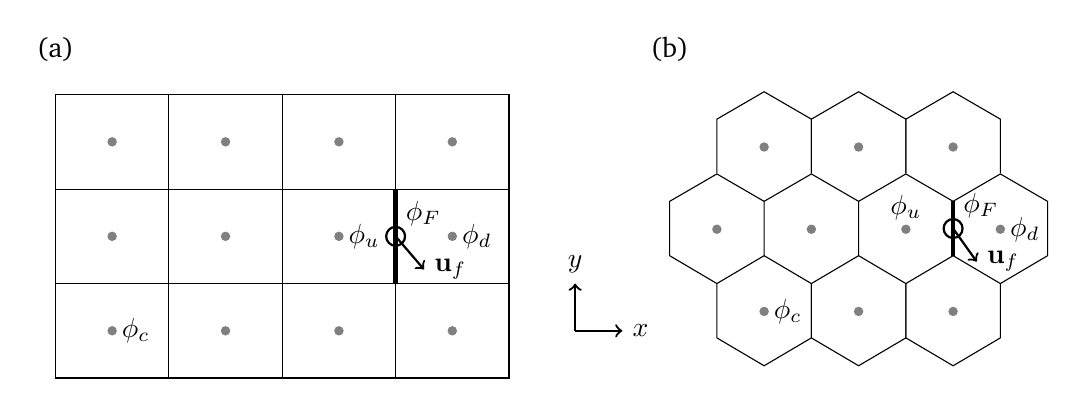
\begin{tikzpicture}[
  scale=0.6,
  cpnt/.style={fill=gray},
]

\begin{scope}[shift={(11,0)}]
	\draw [thick, ->] (0,1) -- (0,2) node [at end, anchor=south] {$y$};
	\draw [thick, ->] (0,1) -- (1,1) node [at end, anchor=west] {$x$};
\end{scope}

\node [above] at (0,6.5) {(a)};
\draw (0,0) rectangle (9.6,6);
\draw (0,2) -- (9.6,2);
\draw (0,4) -- (9.6,4);
\draw (0,0) -- (0,6);
\draw (2.4,0) -- (2.4,6);
\draw (4.8,0) -- (4.8,6);
\draw (7.2,0) -- (7.2,6);

\draw [ultra thick] (7.2,2) -- (7.2,4);
\draw [thick] (7.2,3) circle [radius=0.2] node [anchor=south west] {$\phi_F$};
\draw [thick, ->] (7.2,3) -- (7.8,2.3) node [anchor=west] {$\uf$};

\path [cpnt] (1.2,1) circle [radius=0.1] node [right] {$\phi_c$};
\path [cpnt] (1.2,3) circle [radius=0.1];
\path [cpnt] (1.2,5) circle [radius=0.1];

\path [cpnt] (3.6,1) circle [radius=0.1];
\path [cpnt] (3.6,3) circle [radius=0.1];
\path [cpnt] (3.6,5) circle [radius=0.1];

\path [cpnt] (6.0,1) circle [radius=0.1];
\path [cpnt] (6.0,3) circle [radius=0.1] node [right] {$\phi_u$};
\path [cpnt] (6.0,5) circle [radius=0.1];

\path [cpnt] (8.4,1) circle [radius=0.1];
\path [cpnt] (8.4,3) circle [radius=0.1] node [right] {$\phi_d$};
\path [cpnt] (8.4,5) circle [radius=0.1];

\begin{scope}[shift={(13,2)}]
	\node [above] at (0,4.5) {(b)};

	\draw (1,0) -- (0,0.59) -- (0,1.74) -- (1,2.32) -- (2,1.74) -- (2,0.59) -- (1,0); \path [cpnt] (1,1.15) circle [radius=0.1];
	\draw (2,1.74) -- (3,2.32) -- (4,1.74) -- (4,0.59) -- (3,0) -- (2,0.59); \path [cpnt] (3,1.15) circle [radius=0.1];
	\draw (4,1.74) -- (5,2.32) -- (6,1.74) -- (6,0.59) -- (5,0) -- (4,0.59); \path [cpnt] (5,1.15) circle [radius=0.1] node [above] {$\phi_u$};
	\draw (6,1.74) -- (7,2.32) -- (8,1.74) -- (8,0.59) -- (7,0) -- (6,0.59); \path [cpnt] (7,1.15) circle [radius=0.1] node [right] {$\phi_d$};

	\begin{scope}[shift={(1,-1.74)}]\draw (2,1.74) --(2,0.59) -- (1,0) -- (0,0.59) -- (0,1.74); \path [cpnt] (1,1.15) circle [radius=0.1] node [right] {$\phi_c$};\end{scope}
	\begin{scope}[shift={(3,-1.74)}]\draw (2,1.74) --(2,0.59) -- (1,0) -- (0,0.59) -- (0,1.74); \path [cpnt] (1,1.15) circle [radius=0.1];\end{scope}
	\begin{scope}[shift={(5,-1.74)}]\draw (2,1.74) --(2,0.59) -- (1,0) -- (0,0.59) -- (0,1.74); \path [cpnt] (1,1.15) circle [radius=0.1];\end{scope}

	\begin{scope}[shift={(1,1.74)}]\draw (0,0.59) -- (0,1.74) -- (1,2.32) -- (2,1.74) -- (2,0.59); \path [cpnt] (1,1.15) circle [radius=0.1];\end{scope}
	\begin{scope}[shift={(3,1.74)}]\draw (0,0.59) -- (0,1.74) -- (1,2.32) -- (2,1.74) -- (2,0.59); \path [cpnt] (1,1.15) circle [radius=0.1];\end{scope}
	\begin{scope}[shift={(5,1.74)}]\draw (0,0.59) -- (0,1.74) -- (1,2.32) -- (2,1.74) -- (2,0.59); \path [cpnt] (1,1.15) circle [radius=0.1];\end{scope}

	\draw [ultra thick] (6,0.59) -- (6,1.74);
	\draw [thick] (6,1.165) circle [radius=0.2] node [anchor=south west] {$\phi_F$};
	\draw [thick, ->] (6,1.165) -- (6.5,0.465) node [anchor=west] {$\uf$};
\end{scope}

\end{tikzpicture}
\end{document}

	\caption{Upwind-biased stencils for faces far away from the boundaries of two-dimensional (a) rectangular and (b) hexagon meshes.  The stencil is used to fit a multidimensional polynomial to cell centre values, $\phi_c$, marked by grey circles, in order to approximate the value $\phi_F$ at the face centroid marked by an open circle.  $\phi_u$ and $\phi_d$ are the values at the centroids of the upwind and downwind cells neighbouring the target face, drawn with a heavy line.  The velocity vector $\uf$ is prescribed at face $f$ and determines the choice of stencil at each time-step.}
	\label{fig:cubicFit:interiorStencils}
\end{figure}

The cubicFit scheme approximates the value of the dependent variable at the face, $\phi_F$, using a least-squares fit over a stencil of surrounding known values.
To introduce the approximation method, we will consider how an approximate value is calculated for a face that is far away from the boundaries of a two-dimensional uniform rectangular mesh.
For any mesh, every interior face connects two adjacent cells.  The velocity direction at the face determines which of the two adjacent cells is the upwind cell.  Since the stencil is upwind-biased and asymmetric, two stencils must be constructed for every interior face, and the appropriate stencil is chosen depending on the velocity direction at each face for every time-step.

The upwind-biased stencil for a face $f$ is shown in figure~\ref{fig:cubicFit:interiorStencils}a.  The wind at the face, $\uf$, is blowing from the upwind cell $c_u$ to the downwind cell $c_d$.
To obtain an approximate value at $f$, a polynomial least-squares fit is calculated using the stencil values.
The stencil has \num{4} points in $x$ and \num{3} points in $y$, leading to a natural choice of polynomial that is cubic in $x$ and quadratic in $y$,
\begin{align}
	\phi = a_1 + a_2 x + a_3 y + a_4 x^2 + a_5 xy + a_6 y^2 + a_7 x^3 + a_8 x^2 y + a_9 x y^2 \label{eqn:cubicFit:fullPoly} \text{ .}
\end{align}
A least-squares approach is needed because the system of equations is overconstrained, with \num{12} stencil values but only \num{9} polynomial terms.  The stencil geometry is expressed in a local coordinate system with the face centroid as the origin so that the approximated value $\phi_F$ is equal to the constant coefficient $a_1$.
The stencil is upwind-biased to improve numerical stability, and the multidimensional cubic polynomial is chosen to improve accuracy in the direction of flow \citep{leonard1993}.

The remainder of this \TODO{subsection} generalises the approximation technique for arbitrary meshes and describes the methods for constructing stencils, performing a least-squares fit with a suitable polynomial, and ensuring numerical stability of the transport scheme.

\subsection{Stencil construction}
\label{sec:cubicFit:stencil}

For every interior face, two stencils are constructed, one for each of the possible upwind cells.
Stencils are not constructed for boundary faces because values of $\phi$ at boundaries are calculated from prescribed boundary conditions.
For a given interior face $f$ and upwind cell $c_u$, we find those faces that are connected to $c_u$ and `oppose' face $f$.  These are called the \textit{opposing faces}.
The opposing faces for face $f$ and upwind cell $c_u$ are determined as follows.
Defining $G$ to be the set of faces other than $f$ that border cell $c_u$, we calculate the `opposedness', $\Opp$, between faces $f$ and $g \in G$, defined as
\begin{align}
	\Opp(f, g) \equiv - \frac{\Sf \cdot \vect{S}_g}{\magSf^2} \label{eqn:cubicFit:opp}
\end{align}
where $\Sf$ and $\vect{S}_g$ are the surface area vectors pointing outward from cell $c_u$ for faces $f$ and $g$ respectively.
Using the fact that $\vect{a} \cdot \vect{b} = \Mag{\vect{a}}\:\Mag{\vect{b}} \cos(\theta)$ we can rewrite equation~\eqref{eqn:cubicFit:opp} as
\begin{align}
	\Opp(f, g) = - \frac{\Mag{\vect{S}_g}}{\magSf} \cos(\theta)
\end{align}
where $\theta$ is the angle between faces $f$ and $g$.  In this form, it can be seen that $\Opp$ is a measure of the relative area of $g$ and how closely it parallels face $f$.

The set of opposing faces, $\mathrm{OF}$, is a subset of $G$, comprising those faces with $\Opp \geq 0.5$, and the face with the maximum opposedness.  Expressed in set notation, this is
\begin{align}
	\mathrm{OF}(f,c_u) \equiv \{ g : \Opp(f, g) \geq 0.5 \} \cup \{ g : \max_{g\:\in\:G}(\Opp(f, g)) \} \text{ .}
\end{align}
On a rectangular mesh, there is always one opposing face $g$, and it is exactly parallel to the face $f$ such that $\Opp(f, g) = 1$.

Once the opposing faces have been determined, the set of internal and external cells must be found.  The \textit{internal cells} are those cells that are connected to the opposing faces.  Note that $c_u$ is always an internal cell.  The \textit{external cells} are those cells that share vertices with the internal cells.  Note that $c_d$ is always an external cell.  Finally, the \textit{stencil boundary faces} are boundary faces having Dirichlet boundary conditions\footnote{Boundary faces with Neumann boundary conditions would require extrapolated boundary values to be calculated.
This would create a feedback loop in which boundary values are extrapolated from interior values, then interior values are transported using stencils that include boundary values.  
We have not considered how such an extrapolation could be made consistent with the multidimensional polynomial reconstruction.
Hence, boundary faces with Neumann boundary conditions are excluded from the set of stencil boundary faces.} that share a vertex with the internal cells.
Having found these three sets, the stencil is constructed to comprise all internal cells, external cells and stencil boundary faces.

\begin{figure}
	\centering
	\documentclass[tikz]{standalone}
\newcommand{\iu}{{i\mkern1mu}}
\newcommand{\vect}{\mathbf}
\newcommand{\unitg}{\vect{\hat{g}}}
\newcommand{\unitn}{\vect{\hat{n}}}
\newcommand{\uf}{\vect{u}_f}
\newcommand{\Opp}{\mathrm{Opp}}
\newcommand{\Sf}{\vect{S}_f}
\newcommand{\Mag}[1]{\lvert #1 \rvert}
\newcommand{\magSf}{\Mag{\Sf}}
\newcommand{\area}{\mathcal{A}}
\newcommand{\vol}{\mathcal{V}}
\newcommand{\volave}[1]{\langle #1 \rangle_\vol}
\newcommand{\moment}{\mathfrak{m}}
\newcommand{\rhoexp}{\mathfrak{n}}

\usetikzlibrary{plotmarks}
\usetikzlibrary{patterns}
\begin{document}
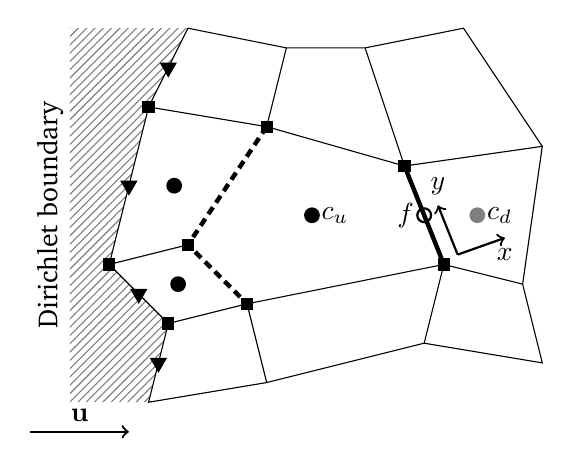
\begin{tikzpicture}[
  scale=0.25,
  cpnt/.style={fill=black},
]
\fill [pattern=north east lines,pattern color=gray] (5,0) -- (6,4) -- (3,7) -- (5, 15) -- (7,19) -- (1,19) -- (1,0);
\node at (0,9.5) {\rotatebox{90}{Dirichlet boundary}};

\draw [white] (-1,-2.1) rectangle (-1,-2);
\draw [thick, ->] (-1,-1.5) -- (4,-1.5) node [midway, anchor=south] {$\vect{u}$};

\draw [thick, ->] (20.7,7.5) -- (19.7,10) node [at end, anchor=south] {$y$};
\draw [thick, ->] (20.7,7.5) -- (23.1,8.35) node [at end, anchor=north] {$x$};

\draw (10,5) -- (20,7) -- (18,12) -- (11,14);
\draw [densely dashed, ultra thick] (11,14) -- (7,8) -- (10,5);
\draw [ultra thick] (20,7) -- (18,12);
\draw [thick] (19,9.5) circle [radius=0.35] node [anchor=east] {$f$};
\path [cpnt] (13.3,9.5) circle [radius=0.4] node [anchor=west, black] {$c_u$};
\path [fill=gray] (21.7,9.5) circle [radius=0.4] node [anchor=west, black] {$c_d$};

% direct upwind cells
\draw (10,5) -- (6,4) -- (3,7) -- (7,8);
\path [cpnt] (6.5,6) circle [radius=0.4];

\draw (3,7) -- (5,15) -- (11,14);
\path [cpnt] (6.3,11) circle [radius=0.4];

\draw (20,7) -- (24,6) -- (25,13) -- (18,12);
\draw (20,7) -- (19,3) -- (25,2) -- (24,6);
\draw (19,3) -- (11,1) -- (10,5);
\draw (11,14) -- (12,18) -- (16,18) -- (18,12);
\draw (16,18) -- (21,19) -- (25,13);
\draw (5,15) -- (7,19) -- (12,18);
\draw (6,4) -- (5,0) -- (11,1);

% vertices
\node at (3,7) {\pgfuseplotmark{square*}};
\node at (5,15) {\pgfuseplotmark{square*}};
\node at (11,14) {\pgfuseplotmark{square*}};
\node at (18,12) {\pgfuseplotmark{square*}};
\node at (10,5) {\pgfuseplotmark{square*}};
\node at (20,7) {\pgfuseplotmark{square*}};
\node at (6,4) {\pgfuseplotmark{square*}};
\node at (7,8) {\pgfuseplotmark{square*}};
\node at (5.5,2) [scale=1.5,rotate=60] {\pgfuseplotmark{triangle*}};
\node at (6,17) [scale=1.5,rotate=60] {\pgfuseplotmark{triangle*}};
\node at (4,11) [scale=1.5,rotate=60] {\pgfuseplotmark{triangle*}};
\node at (4.5,5.5) [scale=1.5,rotate=60] {\pgfuseplotmark{triangle*}};
\end{tikzpicture}
\end{document}

%	\includegraphics{../fig-double-upwind-stencil/fig-double-upwind-stencil.pdf}
	%
	\caption{A fourteen-point, upwind-biased stencil for face $f$ connecting the pentagonal upwind cell, $c_u$, and the downwind cell $c_d$.  The dashed lines denote the two faces of cell $c_u$ that oppose $f$, and black circles mark the centroids of the internal cells that are connected to these two opposing faces.  The stencil is extended outwards by including cells that share vertices with the three internal cells, where black squares mark these vertices.  Four stencil boundary faces, marked by black triangles, are also included.
The local coordinate system $(x, y)$ has its origin at the centroid of face $f$, marked by an open circle, with $x$ normal to $f$ and $y$ perpendicular to $x$.}
	\label{fig:double-upwind-stencil}
\end{figure}

Figure~\ref{fig:double-upwind-stencil} illustrates a stencil construction for face $f$ connecting upwind cell $c_u$ and downwind cell $c_d$.  The two opposing faces are denoted by thick dashed lines and the centres of the three adjoining internal cells are marked by black circles.  The stencil is extended outwards by including the external cells that share vertices with the internal cells, where the vertices are marked by black squares.  A boundary at the far left has Dirichlet boundary conditions, and so the four stencil boundary faces are also included in the stencil, where the boundary face centres are marked by black triangles.  The resultant stencil contains fourteen points.

\subsection{Least-squares fit}
To approximate the value of $\phi$ at a face $f$, a least-squares fit is calculated from a stencil of surrounding known values.  First, we will show how a polynomial least-squares fit is calculated for a face on a rectangular mesh.  Second, we will make modifications to the least-squares fit that are necessary for numerical stability.  

For faces that are far away from the boundaries of a rectangular mesh, we fit the multidimensional polynomial given by equation~\eqref{eqn:cubicFit:fullPoly} that has nine unknown coefficients, $\vect{a} = a_1 \ldots a_9$, using the twelve cell centre values from the upwind-biased stencil, $\bm{\phi} = \phi_1 \ldots \phi_{12}$.  This yields a matrix equation
\begin{align}
	\begin{bmatrix}
		1 & x_1 & y_1 & x_1^2 & x_1 y_1 & y_1^2 & x_1^3 & x_1^2 y_1 & x_1 y_1^2 \\
		1 & x_2 & y_2 & x_2^2 & x_2 y_2 & y_2^2 & x_2^3 & x_2^2 y_2 & x_2 y_2^2 \\
		\vdots & \vdots & \vdots & \vdots & \vdots & \vdots & \vdots & \vdots & \vdots \\
		1 & x_{12} & y_{12} & x_{12}^2 & x_{12} y_{12} & y_{12}^2 & x_{12}^3 & x_{12}^2 y_{12} & x_{12} y_{12}^2 \\
	\end{bmatrix}
	\begin{bmatrix}
		a_1 \\
		a_2 \\
		\vdots \\
		a_9
	\end{bmatrix}
	=
	\begin{bmatrix}
		\phi_1 \\
		\phi_2 \\
		\vdots \\
		\phi_{12}
	\end{bmatrix}
\end{align}
which can be written as
\begin{align}
	\vect{B} \vect{a} = \bm{\phi} \label{eqn:cubicFit:unweightedLeastSquares} \text{ .}
\end{align}
The rectangular matrix $\vect{B}$ has one row for each cell in the stencil and one column for each term in the polynomial.  $\vect{B}$ is called the \textit{stencil matrix}, and it is constructed using only the mesh geometry.
A local coordinate system is established in which $x$ is normal to the face $f$ and $y$ is perpendicular to $x$.
The coordinates $(x_i, y_i)$ give the position of the centroid of the $i$th cell in the stencil.
A two-dimensional stencil is also used for the tests on spherical meshes in section~\ref{sec:cubicFit:deformationSphere}.  In these tests, cell centres are projected perpendicular to a tangent plane at the face centre.  Previous studies found that results were largely insensitive to the projection method \citep{skamarock-gassmann2011,lashley2002}.

The unknown coefficients $\vect{a}$ are calculated using the pseudo-inverse, $\vect{B}^+$, found by singular value decomposition,
\begin{align}
	\vect{a} = \vect{B}^+ \bm{\phi} \text{ .}
%
\intertext{Recall that the approximate value $\phi_F$ is equal to the constant coefficient $a_1$, which is a weighted mean of $\bm{\phi}$,} 
%
	a_1 = \begin{bmatrix}
		b_{1,1}^+ \\
		b_{1,2}^+ \\
		\vdots \\
		b_{1,12}^+
	\end{bmatrix}
	\cdot
	\begin{bmatrix}
		\phi_1 \\
		\phi_2 \\
		\vdots \\
		\phi_{12}
	\end{bmatrix} \label{eqn:cubicFit:weighted-sum}
\end{align}
where the weights $b_{1,1}^+ \ldots b_{1,12}^+$ are the elements of the first row of $\vect{B}^+$.
Note that the majority of the least-squares fit procedure depends on the mesh geometry only.  An implementation may precompute the pseudo-inverse for each stencil during model initialisation, and only the first row needs to be stored.  Since each face has two possible stencils depending on the orientation of the velocity relative to the face, the implementation stores two sets of weights for each face.
Knowledge of the values of $\bm{\phi}$ is only required to calculate the weighted mean given by equation~\eqref{eqn:cubicFit:weighted-sum}, which is evaluated once per face per time-stage.

In the least-squares fit presented above, all stencil values contributed equally to the polynomial fit.
It is necessary for numerical stability that the polynomial fits the cells connected to face $f$ more closely than other cells in the stencil, as shown by \citet{lashley2002,skamarock-menchaca2010}.
To achieve this, we allow each cell to make an unequal contribution to the least-squares fit.
We assign an integer \textit{multiplier} to each cell in the stencil, $\vect{m} = m_1 \ldots m_{12}$, and multiply equation~\eqref{eqn:cubicFit:unweightedLeastSquares} to obtain
\begin{align}
	\vect{\tilde{B}} \vect{a} = \vect{m} \cdot \bm{\phi}
\end{align}
where $\vect{\tilde{B}} = \vect{M} \vect{B}$ and $\vect{M} = \mathrm{diag}(\vect{m})$.  The constant coefficient $a_1$ is calculated from the pseudo-inverse, $\vect{\tilde{B}}^+$,
\begin{align}
	a_1 = \vect{\tilde{b}_1^+} \cdot \vect{m} \cdot \bm{\phi} \label{eqn:cubicFit:weightedPinv}
\end{align}
where $\vect{\tilde{b}_1^+} = \tilde{b}_{1,1}^+ \ldots \tilde{b}_{1,12}^+$ are the elements of the first row of $\vect{\tilde{B}}^+$.
Again, $a_1$ is a weighted mean of $\bm{\phi}$, where the weights are now $\vect{\tilde{b}_1^+} \cdot \vect{m}$.  Values for $\vect{m}$ are chosen so that the cells connected to face $f$ make a greater contribution to the least-squares fit, as discussed later in section~\ref{sec:cubicFit:stabilisation}.

For faces of a non-rectangular mesh, or faces that are near a boundary, the number of stencil points and number of polynomial terms may differ: a stencil will have one or more cells and, for two-dimensional meshes, its polynomial will have between one and nine terms.  Additionally, the polynomial cannot have more terms than its stencil has cells because this would lead to an underconstrained system of equations.  The procedure for choosing suitable polynomials is discussed next.

\subsection{Polynomial generation}
\label{sec:cubicFit:polyGen}

\begin{figure}
	\centering
	\documentclass[tikz]{standalone}
\newcommand{\iu}{{i\mkern1mu}}
\newcommand{\vect}{\mathbf}
\newcommand{\unitg}{\vect{\hat{g}}}
\newcommand{\unitn}{\vect{\hat{n}}}
\newcommand{\uf}{\vect{u}_f}
\newcommand{\Opp}{\mathrm{Opp}}
\newcommand{\Sf}{\vect{S}_f}
\newcommand{\Mag}[1]{\lvert #1 \rvert}
\newcommand{\magSf}{\Mag{\Sf}}
\newcommand{\area}{\mathcal{A}}
\newcommand{\vol}{\mathcal{V}}
\newcommand{\volave}[1]{\langle #1 \rangle_\vol}
\newcommand{\moment}{\mathfrak{m}}
\newcommand{\rhoexp}{\mathfrak{n}}

\usetikzlibrary{patterns}
\begin{document}
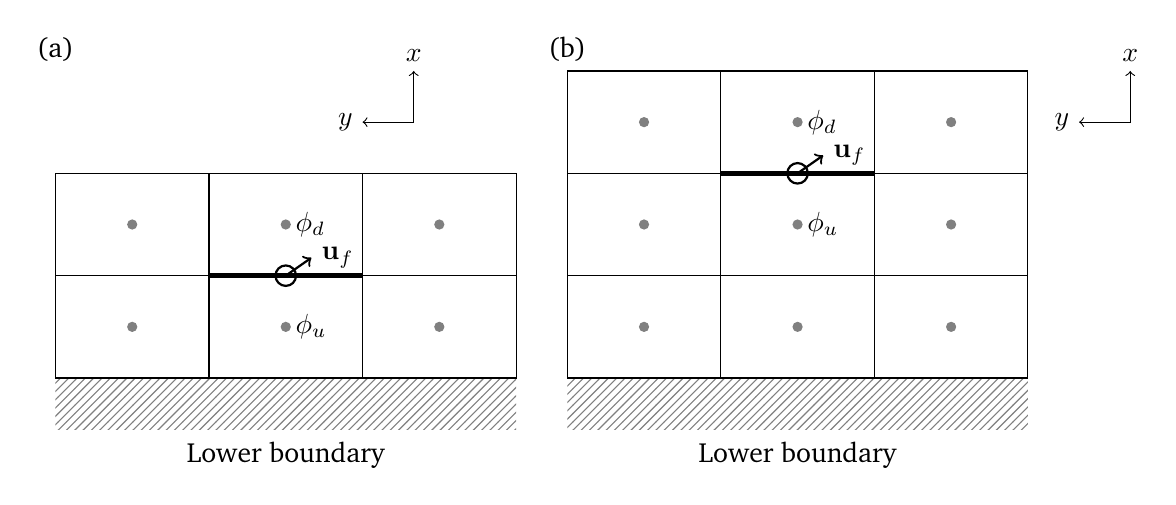
\begin{tikzpicture}[
  scale=0.65,
  cpnt/.style={fill=gray},
]

\node [above] at (0,6) {(a)};
\fill [pattern=north east lines,pattern color=gray] (0,-1) rectangle (9,0);
\node at (4.5,-1.5) {Lower boundary};
\draw (0,0) rectangle (9,4);
\draw (3,0) -- (3,4);
\draw (6,0) -- (6,4);
\draw (0,2) -- (9,2);

\draw [ultra thick] (3,2) -- (6,2);
\draw [thick] (4.5,2) circle [radius=0.2];

\path [cpnt] (1.5,1) circle [radius=0.1];
\path [cpnt] (4.5,1) circle [radius=0.1] node [right] {$\phi_u$};
\path [cpnt] (7.5,1) circle [radius=0.1];
\path [cpnt] (1.5,3) circle [radius=0.1];
\path [cpnt] (4.5,3) circle [radius=0.1] node [right] {$\phi_d$};
\path [cpnt] (7.5,3) circle [radius=0.1];
\draw [thick, ->] (4.5,2) -- (5,2.35) node [anchor=west] {$\uf$};

\draw [<->] (6,5) node [left] {$y$} -- (7,5) -- (7,6) node [above] {$x$};

\begin{scope}[shift={(10,0)}]
\node [above] at (0,6) {(b)};
\fill [pattern=north east lines,pattern color=gray] (0,-1) rectangle (9,0);
\node at (4.5,-1.5) {Lower boundary};
\draw (0,0) rectangle (9,6);
\draw (3,0) -- (3,6);
\draw (6,0) -- (6,6);
\draw (0,2) -- (9,2);
\draw (0,4) -- (9,4);

\draw [ultra thick] (3,4) -- (6,4);
\draw [thick] (4.5,4) circle [radius=0.2];

\path [cpnt] (1.5,1) circle [radius=0.1];
\path [cpnt] (4.5,1) circle [radius=0.1];
\path [cpnt] (7.5,1) circle [radius=0.1];
\path [cpnt] (1.5,3) circle [radius=0.1];
\path [cpnt] (4.5,3) circle [radius=0.1] node [right] {$\phi_u$};
\path [cpnt] (7.5,3) circle [radius=0.1];
\path [cpnt] (1.5,5) circle [radius=0.1];
\path [cpnt] (4.5,5) circle [radius=0.1] node [right] {$\phi_d$};
\path [cpnt] (7.5,5) circle [radius=0.1];
\draw [thick, ->] (4.5,4) -- (5,4.35) node [anchor=west] {$\uf$};

\draw [<->] (10,5) node [left] {$y$} -- (11,5) -- (11,6) node [above] {$x$};
\end{scope}

\end{tikzpicture}
\end{document}

	\caption{Upwind-biased stencils for faces near the lower boundary of a rectangular $x$--$z$ mesh, with (a) a $3 \times 2$ stencil for the face immediately adjacent to the lower boundary, and (b) a $3 \times 3$ stencil for the face immediately adjacent to the face in (a).  Each stencil belongs to the face marked by a thick line.  The local coordinate system is shown, having an $x$ direction normal to the face a $y$ direction tangent to the face.  For both stencils, attempting a least-squares fit using the nine-term polynomial in equation~\eqref{eqn:cubicFit:fullPoly} would result in an underconstrained problem.
	There is no normal flow at the lower boundary.}
	\label{fig:cubicFit:boundaryStencils}
\end{figure}

The majority of faces on a uniform two-dimensional mesh have stencils with more than nine cells.  For example, a rectangular mesh has 12 points (figure~\ref{fig:cubicFit:interiorStencils}a), and a hexagonal mesh has 10 points (figure~\ref{fig:cubicFit:interiorStencils}b).
In both cases, constructing a system of equations using the nine-term polynomial in equation~\eqref{eqn:cubicFit:fullPoly} leads to an overconstrained problem that can be solved using least-squares.
However, this is not true for faces near boundaries: stencils that have fewer than nine cells (figure~\ref{fig:cubicFit:boundaryStencils}a) would result in an underconstrained problem, and stencils that have exactly nine cells may lack sufficient information to constrain high-order terms.
For example, the stencil in figure~\ref{fig:cubicFit:boundaryStencils}b lacks sufficient information to fit the $x^3$ term.  In such cases, it becomes necessary to perform a least-squares fit using a polynomial with fewer terms.

For every stencil, we find a set of \textit{candidate polynomials} that do not result in an underconstrained problem.
In two dimensions, a candidate polynomial has some combination of between one and nine terms from equation~\eqref{eqn:cubicFit:fullPoly}.  There are two additional constraints that a candidate polynomial must satisfy.

First, high-order terms may be included in a candidate polynomial only if the lower-order terms are also included.
More precisely, let
\begin{align}
	M(x, y) = { x^i y^j : i,j \geq 0 \text{ and } i \leq 3 \text{ and } j \leq 2 \text{ and } i+j \leq 3}
\end{align}
be the set of all monomials of degree at most \num{3} in $x, y$.
A subset $S$ of $M(x,y)$ is ``dense'' if, whenever $x^a y^b$ is in $S$, then $x^i y^j$ is also in $S$ for all $0 \leq i \leq a$, $0 \leq j \leq b$.
For example, the polynomial $\phi = a_1 + a_2 x + a_3 y + a_4 xy + a_5 x^2 + a_6 x^2 y$ is a dense subset of $M(x,y)$, but $\phi = a_1 + a_2 x + a_3 y + a_4 x^2 y$ is not because $x^2 y$ can be included only if $xy$ and $x^2$ are also included.
In total there are 26 dense subsets of the two-dimensional polynomial in equation~\eqref{eqn:cubicFit:fullPoly}.

Second, a candidate polynomial must have a stencil matrix $\vect{B}$ that is full rank.  The matrix is considered full rank if its smallest singular value is greater than \num{1e-9}.
Using a polynomial with all nine terms and the stencil in figure~\ref{fig:cubicFit:boundaryStencils}b results in a rank-deficient matrix and so the nine-term polynomial is not a candidate polynomial.

The candidate polynomials are all the dense subsets of $M(x,y)$ that have a cardinality greater than one with a stencil matrix that is full rank.  The final stage of the cubicFit transport scheme selects a candidate polynomial and ensures that the least-squares fit is numerically stable.

\subsection{Stabilisation procedure}
\label{sec:cubicFit:stabilisation}
So far, we have constructed a stencil and found a set of candidate polynomials.  Applying a least-squares fit to any of these candidate polynomials avoids creating an underconstrained problem.  The final stage of the transport scheme chooses a suitable candidate polynomial and appropriate multipliers $\vect{m}$ so that the fit is numerically stable.

The approximated value $\phi_F$ is equal to $a_1$ which is calculated from equation~\eqref{eqn:cubicFit:weightedPinv}.  The value of $a_1$ is a weighted mean of $\bm{\phi}$ where $\vect{w} = \vect{\tilde{b}_1^+} \cdot \vect{m}$ are the weights.
If the cell centre values $\bm{\phi}$ are assumed to approximate a smooth field then we expect $\phi_F$ to be close to the values of $\phi_u$ and $\phi_d$, and expect $\phi_F$ to be insensitive to small changes in $\bm{\phi}$.
When the weights $\vect{w}$ have large magnitude then this is no longer true: $\phi_F$ becomes sensitive to small changes in $\bm{\phi}$ which can result in large, numerically unstable departures from the smooth field $\bm{\phi}$.

To avoid numerical instabilities, a simplified, one-dimensional von Neumann analysis was performed, presented in appendix A.  The analysis is used to impose three stability conditions on the weights $\vect{w}$,
\begin{subequations}
\label{eqn:cubicFit:stability}
\begin{align}
	0.5 \leq w_u \leq 1 \label{eqn:cubicFit:stabilityU} \\
	0 \leq w_d \leq 0.5 \label{eqn:cubicFit:stabilityD} \\
	w_u - w_d \geq \max_{p\:\in\:P}(|w_p|)
\end{align}
\end{subequations}
where $w_u$ and $w_d$ are the weights for the upwind and downwind cells respectively.  The \textit{peripheral points} $P$ are the cells in the stencil that are not the upwind or downwind cells, and $w_p$ is the weight for a given peripheral point $p$.
 The upwind, downwind and peripheral weights sum to one such that $w_u + w_d + \sum_{p \in P} w_p = 1$.

The stabilisation procedure comprises three steps.  In the first step, the set of candidate polynomials is sorted in preference order so that candidates with more terms are preferred over those with fewer terms.
If there are multiple candidates with the same number of terms, the minimum singular value of $\vect{B}$ is calculated for each candidate, and an ordering is imposed such that the candidate with the larger minimum singular value is preferred.  This ordering ensures that the preferred candidate is the highest-order polynomial with the most information content.\footnote{Note that singular values are used for two purposes: first, to test if the matrix $\vect{B}$ is full-rank and, second, to impose an ordering on candidates.
We have used the minimum singular value, $\sigma_\mathrm{min}(\vect{B})$, for both purposes.  Alternatively, we could use the condition number, $\mathrm{cond}(\vect{B})$, which is the ratio of smallest to largest singular value.
Experiments revealed that only the candidate ordering was sensitive to the choice of $\sigma_\mathrm{min}$ or $\mathrm{cond}$.
The most suitable choices of singular value calculations could be explored in future.}

In the second step, the most-preferred polynomial is taken from the list of candidates and the multipliers are assigned so that the upwind cell and downwind cell have multipliers $m_u = 2^{10}$ and $m_d = 2^{10}$ respectively, and all peripheral points have multipliers $m_p = 1$.  These multipliers are very similar to those used by \citet{lashley2002}, leading to a well-conditioned matrix $\vect{\tilde{B}}$ and a least-squares fit in which the polynomial passes almost exactly through the upwind and downwind cell centre values.

In the third step, we calculate the weights $\vect{w}$ and evaluate them against the stability conditions given in equation~\eqref{eqn:cubicFit:stability}.
If any condition is violated, the value of $m_d$ is halved and the conditions are evaluated with the new weights.  This step is repeated until the weights satisfy the stability conditions, or $m_d$ becomes smaller than one.  In practice, the conditions are satisified when $m_d$ is either small (between 1 and 4) or equal to $2^{10}$.  The upwind multiplier $m_u$ is fixed at $2^{10}$ and the peripheral multipliers $m_p$ are fixed at \num{1}.  If the conditions are still not satisfied, then we start again from the second step with the next polynomial in the candidate list. 

Finally, if no stable weights are found for any candidate polynomial, we revert to an upwind scheme such that $w_u = 1$ and all other weights are zero.
In our experiments we have not encountered any stencil for which this last resort is required.
Furthermore, our experiments show that the stabilisation procedure only modifies the least squares fit for stencils near boundaries and for stencils in distorted mesh regions.
For stencils in the interior of a uniform rectangular mesh, the least squares fit includes all terms in equation~\eqref{eqn:cubicFit:fullPoly} with $m_u = m_d = 2^{10}$.

\begin{figure}
	\centering
	\input{cubicFit/stabilisation}
	\caption{One-dimensional least-squares fits with a stencil of five points using (a) a cubic polynomial with multipliers $m_u = 1024$, $m_d = 1024$ and $m_p = 1$, (b) a quadratic polynomial with the same multipliers, and (c) a quadratic polynomial with multipliers $m_u = 1024$, $m_d = 1$ and $m_p = 1$.  Notice that the curves in (a) and (b) fit almost exactly through the upwind and downwind points immediately adjacent to the $y$-axis, but in (c) the curve fits almost exactly only through the upwind point immediately to the left of the $y$-axis.  The point data are labelled with their respective weights.
	Points that have failed one of the stability conditions in equation~\eqref{eqn:cubicFit:stability} are marked in red with italicised labels.  The upwind point is located at $(-1, 1.8)$ and the downwind point at $(0.62, 1.9)$, and the peripheral points are at $(-2.8, 2.4)$, $(-1.6, 2.7)$ and $(-1.2, 2.2)$.  The stabilisation procedure (section~\ref{sec:cubicFit:stabilisation}) calculates weights using only $x$ positions, and values of $\phi$ are included here for illustration only.}
	\label{fig:cubicFit:oscillatory1D}
\end{figure}

To illustrate the stabilisation procedure, figure~\ref{fig:cubicFit:oscillatory1D}a presents a one-dimensional example of a cubic polynomial fitted through five points, with the weight at each point printed beside it.
The stabilisation procedure only uses the $x$ positions of these points and does not use the values of $\phi$ themselves.  The $\phi$ values are included here for illustration only.
Hence, for a given set of $x$ positions, the same set of weights are chosen irrespective of the $\phi$ values.

For a one-dimensional cubic polynomial fit, the list of candidate polynomials in preference order is
\begin{align}
	\phi &= a_1 + a_2 x + a_3 x^2 + a_4 x^3 \label{eqn:cubicFit:cubicCandidate} \text{ ,} \\
	\phi &= a_1 + a_2 x + a_3 x^2 \label{eqn:cubicFit:quadCandidate} \text{ ,} \\
	\phi &= a_1 + a_2 x \text{ ,} \\
	\phi &= a_1 \text{ .}
\end{align}
We begin with the cubic equation~\eqref{eqn:cubicFit:cubicCandidate}.  The multipliers are chosen so that the polynomial passes almost exactly through the upwind and downwind points that are immediately to the left and right of the $y$-axis respectively.
The stability condition on the upwind point is violated because $w_u = 1.822 > 1$ (equation~\ref{eqn:cubicFit:stabilityU}).  Reducing the downwind multiplier does not help to satisfy the stability condition, so we start again with the quadratic equation~\eqref{eqn:cubicFit:quadCandidate}, and the new fit is presented in figure~\ref{fig:cubicFit:oscillatory1D}b.
Again, the multipliers are chosen to force the polynomial through the upwind and downwind points, but this violates the stability condition on the downwind point because $w_d = 0.502 > 0.5$ (equation~\ref{eqn:cubicFit:stabilityD}).  This time, however, stable weights are found by reducing $m_d$ to one (figure~\ref{fig:cubicFit:oscillatory1D}c) and these are the weights that will be used to approximate $\phi_F$, where the polynomial intercepts the $y$-axis.

\subsection{Future extension to three dimensions}
All the procedures used in the cubicFit scheme generalise to three dimensions.  The stencil construction procedure described in section~\ref{sec:cubicFit:stencil} creates a stencil with \num{12} cells for a face in the interior of a two-dimensional rectangular mesh.  In three dimensions, the same procedure creates a stencil with $3 \times 12 = 36$ cells.
A three-dimensional stencil has three times as many cells as its two-dimensional counterpart if the mesh has prismatic cells arranged in columns.  Hence, the computational cost during integration increases three-fold when moving from two dimensions to three dimensions.

To extend the least squares fit to three dimensions, the two-dimensional polynomial in equation~\eqref{eqn:cubicFit:fullPoly} is replaced with its three-dimensional counterpart,
\begin{multline}
	\phi = a_1 + a_2 x + a_3 y + a_4 z + a_5 x^2 + a_6 xy + a_7 y^2 + a_8 xz + a_9 yz + a_{10} z^2 + \\ a_{11} x^3 + a_{12} x^2 y + a_{13} x y^2 + a_{14} x^2 z + a_{15} x z^2 + a_{16} y z^2 + a_{17} y^2 z + a_{18} xyz \text{ .} \label{eqn:cubicFit:fullPoly3D}
\end{multline}
The procedure for generating candidate polynomials described in section~\ref{sec:cubicFit:polyGen} results in 26 dense subsets in two dimensions and 842 dense subsets in three dimensions.  Note that the combinatorial explosion of dense subsets in three dimensions does not increase the computational cost during integration.

The stabilisation procedure described in section~\ref{sec:cubicFit:stabilisation} requires further numerical experiments to verify that it is sufficient for three-dimensional flows and arbitrary polyhedral meshes.
An initial three-dimensional test with uniform flow and a uniform Cartesian mesh obtained a numerically stable result.
For stencils in the interior of the domain, the least squares fit includes all polynomial terms in equation~\eqref{eqn:cubicFit:fullPoly3D} with $m_u = m_d = 2^{10}$.
The stabilisation procedure does not modify the least squares fit for these stencils, but we have not explored the three-dimensional extension of cubicFit any further.

\section{Horizontal transport over mountains}
\label{sec:cubicFit:schaerAdvect}

A two-dimensional transport test was developed by \citet{schaer2002} to study the effect of terrain-following coordinate transformations on numerical accuracy.
In this standard test, a tracer is positioned aloft and transported horizontally over wave-shaped mountains.
When terrain-following meshes are used, this test challenges transport schemes because the tracer must cross mesh layers, which acts to reduce numerical accuracy \citep{schaer2002}.
Here we use a more challenging variant of the test that has steeper mountains and highly-distorted terrain-following meshes.
Numerical convergence and numerical error structures are compared using the linearUpwind and cubicFit transport schemes on terrain-following meshes and cut cell meshes.

The domain is defined on a rectangular $x$--$z$ plane that is \SI{300}{\kilo\meter} wide as measured between the outermost cell centres, and \SI{25}{\kilo\meter} high as measured between upper and lower boundary edges.
Boundary conditions are imposed on the tracer density $\phi$ such that $\phi = \SI{0}{\kilo\gram\per\meter\cubed}$ at the inlet boundary, and a zero normal gradient
$\partial \phi / \partial n = \SI{0}{\kilo\gram\per\meter\tothe{4}}$ is imposed at the outlet boundary.  There is no normal flow at the lower and upper boundaries.

The terrain is wave-shaped, specified by the surface elevation $h$ such that
\begin{subequations}
\begin{align}
   h(x) &= h^\star \cos^2 ( \alpha x )
%
\shortintertext{where}
%
   h^\star(x) &= \left\{ \begin{array}{l l}
       h_0 \cos^2 ( \beta x ) & \enskip \text{if $| x | < a$} \\
	0 & \enskip \text{otherwise}
    \end{array} \right.
\end{align}
\end{subequations}
where $a = \SI{25}{\kilo\meter}$ is the mountain envelope half-width, $h_0 = \SI{6}{\kilo\meter}$ is the maximum mountain height, $\lambda = \SI{8}{\kilo\meter}$ is the wavelength, \(\alpha = \pi / \lambda\) and \(\beta = \pi / (2a)\).  Note that, in order to make this test more challenging, the mountain height $h_0$ is double the mountain height used by \citet{schaer2002}.

\TODO{might have already described BTF in a previous chapter}
A basic terrain-following (BTF) mesh is constructed by using the terrain profile to modify the uniform mesh.
The BTF method uses a linear decay function so that mesh layers become horizontal at the top of the model domain \citep{galchen-somerville1975a},
\begin{equation}
	z(x) = \left( H - h(x) \right) \left( z^\star / H \right) + h(x) \label{eqn:btf}
\end{equation}
where $z$ is the geometric height, $H$ is the height of the domain, $h(x)$ is the surface elevation and $z^\star$ is the computational height of a mesh layer.  If there were no terrain then $h = 0$ and $z = z^\star$.

A velocity field is prescribed with uniform horizontal flow aloft and zero flow near the ground,
\begin{align}
	u(z) = u_0 \left\{ \begin{array}{l l}
		1 & \enskip \text{if $z \geq z_2$} \\
		\sin^2 \left( \frac{\pi}{2} \frac{z - z_1}{z_2 - z_1} \right) & \enskip \text{if $z_1 < z < z_2$} \\
		0 & \enskip \text{otherwise}
	\end{array} \right.	
\end{align}
where $u_0 = \SI{10}{\meter\per\second}$, $z_1 = \SI{7}{\kilo\meter}$ and $z_2 = \SI{8}{\kilo\meter}$.
This results in a constant wind above $z_2$, and zero flow at \SI{7}{\kilo\meter} and below.

The discrete velocity field is defined using a streamfunction, \(\Psi\).  Given that \(u = -\partial \Psi / \partial z\), the streamfunction is found by vertical integration of the velocity profile:
\begin{align}
	\Psi(z) &= -\frac{u_0}{2} \left\{ \begin{array}{l l}
		\left( 2z - z_1 - z_2 \right) & \enskip \text{if $z > z_2$} \\
		z - z_1 - \frac{z_2 - z_1}{\pi} \sin \left(\pi \frac{z - z_1}{z_2-z_1}\right) & \enskip \text{if $z_1 < z \leq z_2$} \\
		0 & \enskip \text{if $z \leq z_1$}
	\end{array} \right.
\end{align}

A tracer with density $\phi$ is positioned upstream above the height of the terrain.  It has the shape
\begin{subequations}
\begin{align}
	\phi(x, z) &= \phi_0 \left\{ \begin{array}{l l}
		\cos^2 \left( \frac{\pi r}{2} \right) & \enskip \text{if $r \leq 1$} \\
		0 & \enskip \text{otherwise}
	\end{array} \right.
%
\intertext{with radius $r$ given by}
%
	r &= \sqrt{
		\left( \frac{x - x_0}{A_x} \right)^2 + 
		\left( \frac{z - z_0}{A_z} \right)^2
	}
\end{align}
%
\label{eqn:cubicFit:schaerAdvect:tracer}
\end{subequations}
where $A_x = \SI{25}{\kilo\meter}$, $A_z = \SI{3}{\kilo\meter}$ are the horizontal and vertical half-widths respectively, and $\phi_0 = \SI{1}{\kilogram\per\meter\cubed}$ is the maximum density of the tracer.  At $t = \SI{0}{\second}$, the tracer is centred at $(x_0, z_0) = (\SI{-50}{\kilo\meter}, \SI{12}{\kilo\meter})$ so that the tracer is upwind of the mountain, in the region of uniform flow above $z_2$.

Tests are integrated for \SI{10000}{\second} using s chosen for each mesh so that the maximum Courant number is about \num{0.4}.  This choice yields a time-step that is well below any stability limit, as recommended by \citet{lauritzen2012}.  By the end of integration the tracer is positioned downwind of the mountain.
The analytic solution at $t = \SI{10000}{\second}$ is centred at $(x_0, z_0) = (\SI{50}{\kilo\meter}, \SI{12}{\kilo\meter})$ with its shape unchanged from the initial condition.

\begin{figure}
	\centering
	\begin{subfigure}{\textwidth}
		\input{cubicFit/schaerAdvect/convergence}
		\phantomsubcaption\label{fig:cubicFit:schaerAdvect:convergence:l2}
		\phantomsubcaption\label{fig:cubicFit:schaerAdvect:convergence:linf}
		\phantomsubcaption\label{fig:cubicFit:tfAdvect:convergence:l2}
		\phantomsubcaption\label{fig:cubicFit:tfAdvect:convergence:linf}
	\end{subfigure}
%
	\caption{Numerical convergence of the two-dimensional tracer transport tests over mountains using
	(\subcaptionref{fig:cubicFit:schaerAdvect:convergence:l2}, \subcaptionref{fig:cubicFit:schaerAdvect:convergence:linf}) horizontal and
	(\subcaptionref{fig:cubicFit:tfAdvect:convergence:l2}, \subcaptionref{fig:cubicFit:tfAdvect:convergence:linf}) terrain-following velocity fields.
	$\ell_2$ errors (equation~\ref{eqn:l2-error}) and $\ell_\infty$ errors (equation~\ref{eqn:linf-error}) are marked at mesh spacings between \SI{5000}{\meter} and \SI{250}{\meter} using linearUpwind and cubicFit transport schemes on basic terrain-following and cut cell meshes.}
	\label{fig:cubicFit:schaerAdvect:convergence}
\end{figure}

To assess numerical convergence, a range of mesh spacings are chosen so that $\Delta x \mathbin{:} \Delta z = 2\mathbin{:}1$ to match the original test specification from \citet{schaer2002}.
Tests were performed using the linearUpwind and cubicFit schemes using BTF meshes and cut cell meshes with mesh spacings between $\Delta x = \SI{250}{\meter}$ and $\Delta x = \SI{5000}{\meter}$.
Error norms are calculated by subtracting the analytic solution from the numerical solution,
\begin{align}
	\ell_2 &= \sqrt{\frac{\sum_c \left(\phi - \phi_T \right)^2 \vol_c}{\sum_c \left(\phi_T^2 \vol_c \right)}} \label{eqn:l2-error} \\
	\ell_\infty &= \frac{\max_c \Mag{\phi - \phi_T}}{\max_c \Mag{\phi_T}} \label{eqn:linf-error}
\end{align}
where $\phi$ is the numerical value, $\phi_T$ is the analytic value, $\sum_c$ denotes a summation over all cells $c$ in the domain, and $\max_c$ denotes a maximum value of any cell.
The linearUpwind and cubicFit schemes are second-order convergent in the $\ell_2$ norm (figure~\ref{fig:cubicFit:schaerAdvect:convergence:l2}) and $\ell_\infty$ norm (figure~\ref{fig:cubicFit:schaerAdvect:convergence}) at all but the coarsest mesh spacings where errors are saturated for both schemes.

The cubicFit scheme achieves a given $\ell_2$ error using a mesh spacing that is almost twice as coarse as that needed by the linearUpwind scheme.  Doubling the mesh spacing results in a coarser mesh with four times fewer cells because the $\Delta x \mathbin{:} \Delta z$ aspect ratio is fixed.
Recall that the stencil for the cubicFit scheme has about twice as many cells as the stencil for the linearUpwind scheme.
Hence, for a given $\ell_2$ error, the computational cost during integration of the cubicFit scheme is about half the computational cost of the linearUpwind scheme.

\begin{figure}
	\centering
	\begin{subfigure}{\textwidth}
		\centering
		\includegraphics{thesis/cubicFit/schaerAdvect/fig-error.pdf}
		\phantomsubcaption\label{fig:cubicFit:schaerAdvect:error:btf:linearUpwind}
		\phantomsubcaption\label{fig:cubicFit:schaerAdvect:error:cutCell:linearUpwind}
		\phantomsubcaption\label{fig:cubicFit:schaerAdvect:error:btf:cubicFit}
		\phantomsubcaption\label{fig:cubicFit:schaerAdvect:error:cutCell:cubicFit}
		\phantomsubcaption\label{fig:cubicFit:tfAdvect:error:btf:linearUpwind}
		\phantomsubcaption\label{fig:cubicFit:tfAdvect:error:cutCell:linearUpwind}
		\phantomsubcaption\label{fig:cubicFit:tfAdvect:error:btf:cubicFit}
		\phantomsubcaption\label{fig:cubicFit:tfAdvect:error:cutCell:cubicFit}
	\end{subfigure}
	\caption{Tracer contours at the end of integration for the two-dimensional tracer transport tests over mountains using
	(\subcaptionref{fig:cubicFit:schaerAdvect:error:btf:linearUpwind},
	\subcaptionref{fig:cubicFit:schaerAdvect:error:cutCell:linearUpwind},
	\subcaptionref{fig:cubicFit:schaerAdvect:error:btf:cubicFit},
	\subcaptionref{fig:cubicFit:schaerAdvect:error:cutCell:cubicFit}) horizontal and 
	(\subcaptionref{fig:cubicFit:tfAdvect:error:btf:linearUpwind},
	\subcaptionref{fig:cubicFit:tfAdvect:error:cutCell:linearUpwind},
	\subcaptionref{fig:cubicFit:tfAdvect:error:btf:cubicFit},
	\subcaptionref{fig:cubicFit:tfAdvect:error:cutCell:cubicFit}) terrain-following velocity fields.  The numerical solution, marked with solid lines, and the analytic solution, marked with dashed lines, are plotted every \num{0.1}.  Tracer contours overlay a color error field, calculated by subtracting the analytic solution from the numerical solution.  Only the lowest \SI{20}{\kilo\meter} in the lee of the mountain is plotted.  The entire domain is \SI{301}{\kilo\meter} wide and \SI{25}{\kilo\meter} high.
	}
	
	\label{fig:cubicFit:schaerAdvect:error}
\end{figure}

Next, we examine the structure of numerical errors with test results using the linearUpwind and cubicFit transport schemes on BTF and cut cell meshes with $\Delta x = \SI{1000}{\meter}$ and $\Delta z = \SI{500}{\meter}$.
To obtain a maximum Courant number of about \num{0.4}, we choose $\Delta t = \inputval{schaerAdvect-cutCell-1000-linearUpwind/dt}$ on the cut cell mesh where the flow is aligned with mesh layers and there are no fluxes through upper and lower cell faces.
Since there is no flow below $z = \SI{7}{\kilo\meter}$, the time-step is not constrained by small, cut cells next to the lower boundary.
On the BTF mesh, $\Delta t$ is only \inputval{schaerAdvect-btf-1000-linearUpwind/dt} because the flow is misaligned with mesh layers, with fluxes through all four faces of cells above sloping terrain.

The highly-distorted BTF mesh presents a particular challenge to the linearUpwind scheme with the final numerical solution, marked by solid lines, losing its correct shape and maximum intensity compared to the analytic solution marked by dashed lines (figure~\ref{fig:cubicFit:schaerAdvect:error:btf:linearUpwind}).
The linearUpwind scheme produces a much better solution on the cut cell mesh, with only small phase errors apparent in figure~\ref{fig:cubicFit:schaerAdvect:error:cutCell:linearUpwind}.
Accuracy is much improved using the cubicFit scheme: on the BTF mesh, shape and maximum intensity are similar to the analytic solution (figure~\ref{fig:cubicFit:schaerAdvect:error:btf:cubicFit}) and, on the cut cell mesh, numerical errors are so small they are not visible (figure~\ref{fig:cubicFit:schaerAdvect:error:cutCell:cubicFit}).
The numerical and analytic contours overlay a color error field that reveals horizontal streaks of error on the BTF mesh (figure~\ref{fig:cubicFit:schaerAdvect:error:btf:linearUpwind},~\ref{fig:cubicFit:schaerAdvect:error:btf:cubicFit}) that were generated above the steepest mountain peaks before becoming trapped in the region of zero flow below $z = \SI{7}{\kilo\meter}$.

The horizontal transport test demonstrates that the cubicFit scheme is second-order convergent in the domain interior irrespective of mesh distortions.  Numerical errors are largest on terrain-following meshes, due either to misalignment of the flow with mesh layers, or to mesh distortions.
In the next section, we propose a new test in order to identify the primary cause of these numerical errors.

\section{Deformational flow on a sphere}
\label{sec:cubicFit:deformationSphere}

The tests presented so far have used flows that are mostly uniform on meshes that are based on rectangular cells.
To ensure that the cubicFit transport scheme is suitable for complex flows on a variety of meshes, we use a standard test of deformational flow on a spherical Earth, as specified by \citet{lauritzen2012}.  
Results are compared between linearUpwind and cubicFit schemes using hexagonal-icosahedral meshes and cubed-sphere meshes.
Hexagonal-icosahedral meshes are constructed by successive refinement of a regular icosahedron following the approach by \citet{thuburn2014,heikes-randall1995a,heikes-randall1995b} without any mesh twisting.
Cubed-sphere meshes are constructed using an equi-distant gnomic projection of a cube having a uniform Cartesian mesh on each panel \citep{staniforth-thuburn2012}.

Following appendix A9 in \citet{lauritzen2014}, the average equatorial spacing $\Delta \lambda$ is used as a measure of mesh spacing.  It is defined as
\begin{align}
	\Delta \lambda = \ang{360} \frac{\overline{\Delta x}}{2 \pi R_e}
\end{align}
where $\overline{\Delta x}$ is the mean distance between cell centres and $R_e = \SI{6.3712e6}{\meter}$ is the radius of the Earth.

The deformational flow test specified by \citet{lauritzen2012} comprised six elements:
\begin{enumerate}
\item a convergence test using a Gaussian-shaped tracer
\item a ``minimal'' resolution test using a cosine bell-shaped tracer
\item a test of filament preservation
\item a test using a ``rough'' slotted cylinder tracer
\item a test of correlation preservation between two tracers
\item a test using a divergent velocity field
\end{enumerate}
We assess the cubicFit scheme using the first two tests only.  We do not consider filament preservation, correlation preservation, or the transport of a ``rough'' slotted cylinder because no shape-preserving filter has yet been developed for the cubicFit scheme.  Stable results were obtained when testing the cubicFit scheme using a divergent velocity field, but no further analysis is made here.

The first deformational flow test uses an infinitely continuous initial tracer that is transported in a non-divergent, time-varying, rotational velocity field.
The velocity field deforms two Gaussian `hills' of tracer into thin vortical filaments.  Half-way through the integration the rotation reverses so that the filaments become circular hills once again.  The analytic solution at the end of integration is identical to the initial condition.
A rotational flow is superimposed on a time-invariant background flow in order to avoid error cancellation.
The non-divergent velocity field is defined by the streamfunction $\Psi$,
\begin{align}
	\Psi(\lambda, \theta, t) = \frac{10 R_e}{T} \sin^2 \left(\lambda'\right) \cos^2 \left(\theta\right) \cos \left( \frac{\pi t}{T} \right) - \frac{2 \pi R_e}{T} \sin\left(\theta\right)
\end{align}
where $\lambda$ is a longitude, $\theta$ is a latitude, $\lambda' = \lambda - 2 \pi t / T$, and $T = \num{12}$ days is the duration of integration.  The time-step is chosen such that the maximum Courant number is about 0.4.

The initial tracer density $\phi$ is defined as the sum of two Gaussian hills,
\begin{align}
	\phi = \phi_1(\lambda, \theta) + \phi_2(\lambda, \theta) \text{ .}
\end{align}
An individual hill $\phi_i$ is given by
\begin{align}
	\phi_i(\lambda, \theta) = \phi_0 \exp\left( -b \left( \frac{\Mag{\vect{x} - \vect{x}_i}}{R_e} \right)^2 \right)
\end{align}
where $\phi_0 = \SI{0.95}{\kilo\gram\per\meter\cubed}$ and $b = 5$.  The Cartesian position vector $\vect{x} = (x,y,z)$ is related to the spherical coordinates $(\lambda, \theta)$ by
\begin{align}
	(x,y,z) = (R_e \cos \theta \cos \lambda, R_e \cos \theta \sin \lambda, R_e \sin \theta) \label{eqn:cubicFit:spherical-cartesian} \text{ .}
\end{align}
The centre of hill $i$ is positioned at $\vect{x}_i$.  In spherical coordinates, two hills are centred at
\begin{align}
	(\lambda_1,\theta_1) &= (5 \pi /6, 0) \\
	(\lambda_2,\theta_2) &= (7 \pi /6, 0)
\end{align}

\begin{figure}
	\centering
	\begin{subfigure}{0.35\textwidth}
		\caption{$t = \SI{0}{\second}$}
		\label{fig:cubicFit:deformationSphere-evolution:initial}
		\includegraphics{deformationSphere-gaussians-hex-8-cubicFit/0/tracer.pdf}
	\end{subfigure}
	\begin{subfigure}{0.3\textwidth}
		\caption{$t = T/2$}
		\label{fig:cubicFit:deformationSphere-evolution:mid}
		\includegraphics{deformationSphere-gaussians-hex-8-cubicFit/518400/tracerW.pdf}
	\end{subfigure}
	\begin{subfigure}{0.3\textwidth}
		\caption{$t = T$}
		\label{fig:cubicFit:deformationSphere-evolution:final}
		\includegraphics{deformationSphere-gaussians-hex-8-cubicFit/1036800/tracerW.pdf}
	\end{subfigure}
%
	\vspace{0.5em} \\
	\includegraphics[height=5in,angle=270]{deformationSphere-gaussians-hex-8-cubicFit/deformationSphere-gaussiansInitialTracer-colorBar.eps}
%
	\caption{Tracer fields for the deformational flow test using initial Gaussian hills.  The tracer is deformed by the velocity field before the rotation reverses to return the tracer to its original distribution:
	(\subcaptionref{fig:cubicFit:deformationSphere-evolution:initial}) the initial tracer distribution at $t = \SI{0}{\second}$;
	(\subcaptionref{fig:cubicFit:deformationSphere-evolution:mid}) by $t=T/2$ the Gaussian hills are stretched into a thin S-shaped filament;
	(\subcaptionref{fig:cubicFit:deformationSphere-evolution:final}) at $t=T$ the tracer resembles the initial Gaussian hills except for some distortion and diffusion due to numerical errors.  Results were obtained with the cubicFit scheme on a hexagonal-icosahedral mesh with an average equatorial mesh spacing of $\Delta \lambda = \inputval{deformationSphere-mesh-hex-8/averageEquatorialSpacing}$.}
	\label{fig:cubicFit:deformationSphere-evolution}
\end{figure}

The results in figure~\ref{fig:cubicFit:deformationSphere-evolution} are obtained using the cubicFit scheme on a hexagonal-icosahedral mesh with $\Delta \lambda = \inputval{deformationSphere-mesh-hex-8/averageEquatorialSpacing}$.
The initial Gaussian hills are shown in figure~\ref{fig:cubicFit:deformationSphere-evolution:initial}.
At $t=T/2$ the tracer has been deformed into an S-shaped filament (figure~\ref{fig:cubicFit:deformationSphere-evolution:mid}).
By $t=T$ the tracer has almost returned to its original distribution except for some slight distortion and diffusion that are the result of numerical errors (figure~\ref{fig:cubicFit:deformationSphere-evolution:final}).

\begin{figure}
	\centering
	\input{cubicFit/deformationSphere/gaussiansConvergence}
	\caption{Numerical convergence of the deformational flow test on the sphere using initial Gaussian hills.  $\ell_2$ errors (equation~\ref{eqn:l2-error}) and $\ell_\infty$ errors (equation~\ref{eqn:linf-error}) are marked at mesh spacings between \inputval{deformationSphere-mesh-hex-4/averageEquatorialSpacing} and \inputval{deformationSphere-mesh-hex-9/averageEquatorialSpacing} using the linearUpwind scheme (dotted lines) and the cubicFit scheme (solid lines) on hexagonal-icosahedral meshes and cubed-sphere meshes.}
	\label{fig:cubicFit:deformationSphere-gaussian-convergence}
\end{figure}

To determine the order of convergence and relative accuracy of the linearUpwind and cubicFit schemes, the same test was performed at a variety of mesh spacings betweeen $\Delta \lambda = \inputval{deformationSphere-mesh-hex-4/averageEquatorialSpacing}$ and $\Delta \lambda = \inputval{deformationSphere-mesh-hex-9/averageEquatorialSpacing}$ on hexagonal-icosahedral meshes and cubed-sphere meshes.  The results are shown in figure~\ref{fig:cubicFit:deformationSphere-gaussian-convergence}.
The solution is slow to converge at coarse resolutions, and this behaviour agrees with the results from \citet{lauritzen2012}.  Both linearUpwind and cubicFit schemes achieve second-order accuracy at smaller mesh spacings. 
For any given mesh type and mesh spacing, the cubicFit scheme is more accurate than the linearUpwind scheme.
Results are more accurate using hexagonal-icosahedral meshes compared to cubed-sphere meshes.  It is not known whether the larger errors on cubed-sphere meshes are due to mesh non-uniformities at panel corners but there is no evidence of grid imprinting in the error fields (not shown).

A slightly more challenging variant of the same test is performed using a quasi-smooth tracer field defined as the sum of two cosine bells,
\begin{align}
	\phi =
	\begin{cases}
		b + c \phi_1(\lambda, \theta) & \quad \text{if $r_1 < r$,} \\
		b + c \phi_2(\lambda, \theta) & \quad \text{if $r_2 < r$,} \\
		b			      & \quad \text{otherwise.}
	\end{cases}
\end{align}
The velocity field is the same as before.  This test is used to determine the ``minimal'' resolution, $\Delta \lambda_m$, which is specified by \citet{lauritzen2012} as the coarsest mesh spacing for which $\ell_2 \approx 0.033$.

\begin{table}
	\robustify\itshape
	\centering
	\begin{tabular}{l l S[detect-weight, detect-shape, detect-mode, round-mode=off]}
\toprule
	Transport scheme & Mesh type & {Minimal resolution (\si{\degree})} \\
\midrule
	linearUpwind & Cubed-sphere & \itshape 0.15 \\
	\makecell{FARSIGHT, grid-point semi-Lagrangian \\ \quad\citep{white-dongarra2011}} & Cubed-sphere & 0.1875 \\
	linearUpwind & Hexagonal-icosahedral & \itshape 0.2 \\
	\makecell{SLFV-SL, swept-area scheme \\ \quad\citep{miura2007}} & Hexagonal-icosahedral & 0.25 \\
	cubicFit & Cubed-sphere & \itshape 0.25 \\
	cubicFit & Hexagonal-icosahedral & 0.3 \\
	\makecell{ICON-FFSL, swept-area scheme \\ \quad\citep{miura2007}} & Triangular-icosahedral & 0.42 \\
\bottomrule
\end{tabular}
%
	\caption{Minimal resolutions for the cubicFit and linearUpwind schemes in the test of deformational flow using cosine bells.  Italicised values have been extrapolated using the second-order convergence obtained at coarser mesh spacings.  For comparison with existing models, some results are also included for unlimited versions of the transport schemes from the intercomparison by \citet{lauritzen2014}.}
	\label{tab:deformationSphere:minimal-resolution}
\end{table}

The minimal resolution for the cubicFit scheme on a hexagonal-icosahedral mesh is about $\Delta \lambda_m = \ang[round-precision=1]{0.3}$.  Tests were not performed at mesh spacings finer than $\Delta \lambda = \inputval{deformationSphere-mesh-hex-9/averageEquatorialSpacing}$ but approximate minimal resolutions have been extrapolated from the second-order convergence that is found at fine mesh spacings.  These minimal resolutions are presented in table~\ref{tab:deformationSphere:minimal-resolution} along with a selection of transport schemes having similar minimal resolutions from the model intercomparison by \citet{lauritzen2014}.

The series of deformational flow tests presented here demonstrate that the cubicFit scheme is suitable for transport on spherical meshes based on quadrilaterals and hexagons.  The cubicFit scheme is largely insensitive to the mesh type, and results are more accurate compared to the linearUpwind scheme for a given mesh type and mesh spacing.  Neither scheme requires special treatment at the corners of cubed-sphere panels.




\chapter{A new mesh for representing the atmosphere above terrain}
\label{ch:slanted}

\begin{highlights}
{\Large Highlights}
\begin{itemize}
	\item The new slanted cell mesh permits longer time-steps than cut cells, with time-steps comparable to terrain-following meshes
	\item Resting atmosphere simulations are more accurate using the new slanted cell method compared to terrain-following methods
	\item Unlike the multidimensional linear upwind scheme, the cubicFit scheme is numerically stable over very steep slopes
\end{itemize}
\end{highlights}

Two sources of numerical error receive particular attention in atmospheric models: errors associated with transport terms and errors associated with the pressure gradient term.
The previous chapter developed the cubicFit transport scheme that reduces numerical errors associated with transport over mountains.
This chapter seeks to reduce errors associated with the balance between the pressure gradient and gravity by representing the atmosphere above terrain by introducing a new type of mesh, the `slanted cell' mesh.

Pressure gradient errors result in spurious flows that are especially apparent for diurnal valley flows where synoptic-scale winds are weak \citep{fast2003}, and even small velocity errors can produce large errors in derived quantities such as relative vorticity and potential vorticity \citep{hoinka-zaengl2004}.
These numerical errors are particularly large using terrain-following meshes with steeply sloping terrain \citep{zaengl2012}.
Terrain-following meshes are typically implemented using a coordinate transform that introduces metric terms into the equations of motion.  The horizontal pressure gradient $\left. \partial p / \partial x \right|_z$ can be written as \citep{mahrer1984}
\begin{align}
	\left. \frac{\partial p}{\partial x} \right|_z = 
	\left. \frac{\partial p}{\partial x} \right|_{z^\star} +
	\left. \frac{\partial z^\star}{\partial x} \right|_z
	\frac{\partial p}{\partial z^\star} \label{eqn:slanted:dpdx}
\end{align}
where $\left. \partial / \partial x \right|_z$ denotes a horizontal derivative at a fixed height in the physical domain, and $\left. \partial / \partial x \right|_{z^\star}$ denotes a horizontal derivative at a fixed model level in the computational domain, with $z^\star$ held constant.
The first term on the right hand side of equation~\eqref{eqn:slanted:dpdx} is the change in pressure along the terrain-following coordinate surfacee, and the second term corrects for the vertical contribution in the first.
These terms tend to be large and of opposite sign over steep terrain, and cancellation errors between the two terms result in pressure gradients errors that drive spurious flows.

\begin{figure}
	\centering
	\begin{subfigure}{\textwidth}
		\phantomsubcaption\label{fig:slanted:resting:meshes:btf}
		\phantomsubcaption\label{fig:slanted:resting:meshes:sleve}
		\phantomsubcaption\label{fig:slanted:resting:meshes:cutCell}
		\phantomsubcaption\label{fig:slanted:resting:meshes:slantedCell}
		\includegraphics{thesis/slanted/resting/fig-meshes.pdf}
	\end{subfigure}
%
	\caption{Two dimensional $x$-$z$ meshes created with the
	(\subcaptionref{fig:slanted:resting:meshes:btf}) basic terrain-following,
	(\subcaptionref{fig:slanted:resting:meshes:sleve}) SLEVE,
	(\subcaptionref{fig:slanted:resting:meshes:cutCell}) cut cell, and
	(\subcaptionref{fig:slanted:resting:meshes:slantedCell}) slanted cell methods, used for the resting atmosphere tests in section~\ref{sec:slanted:resting}.  Cell edges are marked by thin black lines.  The peak mountain height $h_0 = \SI{6}{\kilo\meter}$.
	Only the central region of the domain is shown.  The entire domain is \SI{201}{\kilo\meter} wide and \SI{20}{\kilo\meter} high.}
	\label{fig:slanted:resting:meshes}
\end{figure}

There are two common approaches to reducing errors associated with terrain-following meshes.
The first approach reduces the influence of the terrain on the mesh by choosing a vertical decay function that smooths mesh layers rapidly with height.
The Smooth Level Vertical (SLEVE) decay function formulated by \citet{schaer2002}, later improved by \citet{leuenberger2010}, is one such approach.
The SLEVE method achieves a less distorted terrain-following mesh in the middle and top of the domain than the BTF method.
The difference is illustrated in figure~\ref{fig:slanted:resting:meshes}, in which the SLEVE mesh (figure~\ref{fig:slanted:resting:meshes:sleve}) is noticeably smoother than the equivalent BTF mesh (figure~\ref{fig:slanted:resting:meshes:btf}).
The terrain height is split into coarse-scale and fine-scale components, \(h_1\) and \(h_2\), such that \(h = h_1 + h_2\), with each component having a different exponential decay.
The transformation is defined as \citep{leuenberger2010}
\begin{align}
	z &= z^\star + h_1 b_1 + h_2 b_2
\intertext{where the vertical decay functions are given by}
	b_i &= \frac{\sinh \left( \left( H / s_i \right)^n - \left( z^\star / s_i \right)^n \right)}{\sinh \left( H / s_i \right)^n}
\end{align}
and \(s_1\) and \(s_2\) are the scale heights of coarse-scale and fine-scale terrain respectively.
The exponent \(n\) was introduced by \citet{leuenberger2010} in order to increase cell thickness in the layers nearest the ground, allowing longer timesteps.  In their experiments, \citet{leuenberger2010} found the exponent to have an optimal value of \(n = 1.35\).  Choosing \(n = 1\) gives the decay functions used by \citet{schaer2002}.
While SLEVE can produce very smooth meshes, the coordinate transform becomes non-monotonic and the SLEVE mesh becomes tangled if parameter values are chosen poorly \citep{schaer2002,leuenberger2010}, making it difficult to produce a very smooth global mesh with real terrain (C. K\"{u}hnlein 2015, personal communication).
Many operational atmospheric models use some form of coordinate smoothing \citep{eckermann2009}, and this approach has been found to reduce pressure gradient errors \citep{schaer2002,leuenberger2010,klemp2011}.

The second approach to reducing pressure gradient errors is to improve the accuracy in calculating the horizontal pressure gradient itself.
Instead of calculating the horizontal pressure gradient in the computational domain, the techniques proposed by \citet{klemp2011} and \citet{zaengl2012} both involve interpolation onto $z$ levels in the physical domain.  This gave them the flexibility to design more accurate horizontal pressure gradient discretizations using more appropriate stencils.

\TODO{Another approach is to improve the balance between pressure gradient and gravity and reduce the spurious solenoidal term by using a curl-free gradient formulation \citep{weller-shahrokhi2014}.  I think I should describe this formulation and explain why errors can grow with increasing non-orthogonality.}

Cut cell meshes are less distorted than any smoothed terrain-following mesh, and some studies have shown examples where cut cells produce more accurate results when compared to terrain-following meshes.
Spurious winds seen using terrain-following meshes are not present with cut cells, and errors do not increase with steeper terrain \citep{good2014}.
A comparison of terrain-following and cut cell meshes using real initial data by \citet{steppeler2013} found that 5-day forecasts of precipitation and wind over Asia in January 1989 were more accurate in the cut-cell model, although this result was dependent on using an old version of a model.
Although cut cell meshes are almost entirely undistorted, when explicit methods are used with cut cells, the small cell problem must be overcome in order to avoid severe time-step constraints.

We seek a new type of mesh that improves the balance between the pressure gradient and gravity compared to terrain-following methods, and avoids the severe time-step constraints associated with arbitrarily small cut cells.  Section~\ref{sec:slanted:method} describes the slanted cell method which is designed to satisfy these criteria.
Section~\ref{sec:slanted:mountainAdvect} presents a new two-dimensional test that challanges transport schemes by transporting a tracer along the ground through slanted cells, and this test is used to measure time-step constraints for terrain-following, cut cell and slanted cell meshes.
Section~\ref{sec:slanted:exnerFoamH} outlines the discretisation of the fully compressible model taken from \citet{weller-shahrokhi2014} which includes a curl-free pressure gradient formulation.
In section~\ref{sec:slanted:resting}, the fully compressible model is used to simulate a standard resting atmosphere test case \citep{klemp2011}, comparing results using terrain-following, cut cell and slanted cell meshes.

\section{Generalising the Charney–Phillips staggering for arbitrary meshes}
\label{sec:cp:method}

The generalisation of the Lorenz staggering for arbitrary meshes is straightforward \citep{weller-shahrokhi2014} but this is not true for the Charney--Phillips staggering, which is only suitable for structured meshes with cells stacked in columns.
On a finite volume mesh, variables are ordinarily placed at cell centres or cell faces.
In the Charney--Phillips staggering, the thermodynamic variable is placed at only those cell faces that lie on the vertical coordinate surfaces, and vertically-oriented faces have no thermodynamic information.
This existing staggering is unsuitable for arbitrary finite volume meshes because faces can have any orientation.

A generalised Charney--Phillips staggering will be particularly relevant to atmospheric models that use vertical mesh refinement techniques.
Mesh refinement has received growing attention in atmospheric modelling literature because it could enable atmospheric models to produce more accurate forecasts with less computation \citep{behrens2006,jablonowski2009}.
While much of the literature concentrates on horizontal mesh refinement, some investigations have been made into vertical refinement on two-dimensional $x$--$z$ Cartesian planes:
\citet{mueller2013} have used conforming refinement of triangular meshes for simulating the standard rising bubble and density current test cases, \citet{vanhooft2018} have used block-structured adaptive mesh refinement for direct numerical simulations of the atmospheric boundary layer, and \citet{yamazaki-satomura2012} have used nonconforming block-refinement to better resolve the atmosphere immediately above idealised mountains.

According to \citet{thuburn-woolings2005}, the vertical discretisation used by \citet{yamazaki-satomura2012} supports computational modes and instabilities, although these errors were not excited by the test cases performed by \citet{yamazaki-satomura2012}.
The Charney--Phillips staggering is not susceptible to such errors, but we are not aware of any existing literature that combines mesh refinement with a Charney--Phillips staggering.
By allowing for any mesh structure, a generalised Charney--Phillips formulation should be suitable for any type of mesh, including conforming and non-conforming mesh refinement, terrain-following meshes, cut cell meshes and slanted cell meshes.

\subsection{Generalised Charney--Phillips formulation}

\begin{figure}
	\centering
	\documentclass[tikz]{standalone}
\usepackage{times}
\usepackage{bm}
\begin{document}
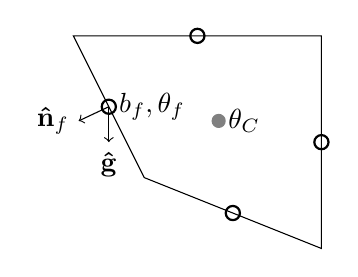
\begin{tikzpicture}[
  scale=0.45,
  cpnt/.style={fill=gray}
]

\draw (2,3) -- (0,7) -- (7,7) -- (7,1) -- (2,3);

\path [cpnt] (4.1,4.6) circle [radius=0.2] node [right] {$\theta_C$};

\draw [thick] (7,4) circle [radius=0.2];
\draw [thick] (4.5,2) circle [radius=0.2];
\draw [thick] (3.5,7) circle [radius=0.2];
\draw [thick] (1,5) circle [radius=0.2] node [right] {$b_f, \theta_f$};

\draw [->] (1,5) -- (0.15,4.6) node [left] {$\mathbf{\hat{n}}_f$};
\draw [->] (1,5) -- (1,4) node [below] {$\mathbf{\hat{g}}$};

\end{tikzpicture}
\end{document}

	\caption{A quadrilateral cell with the prognostic thermodynamic variable $b_f$ stored at face centres marked by open circles.
	$b_f$ is calculated from the potential temperature $\theta_f$ such that $b_f = \theta_f \unitg \cdot \unitn_f$ where $\unitn_f$ is the unit vector outward normal to face $f$, and $\unitg$ is the unit vector of gravitational acceleration.
	The potential temperature at the cell centre, $\theta_C$, is reconstructed from surrounding values of $b_f$ using equation~\eqref{eqn:cp:reconstruct}.}
	\label{fig:cp:staggering}
\end{figure}

The generalised Charney--Phillips model is a new variant of the fully compressible Euler model with a Lorenz staggering, as documented by \citet{weller-shahrokhi2014} and summarised in section~\ref{sec:slanted:exnerFoamH}.
The model variant uses a newly-formulated generalisation of the Charney--Phillips staggering for arbitrary meshes.
The primary difference between the Lorenz and Charney--Phillips formulations is their treatment of the prognostic thermodynamic variable: the generalised Charney--Phillips formulation stores the prognostic thermodynamic variable $b_f$ at all cell faces such that $b_f = \theta_f \unitg \cdot \unitn_f$ where $f$ is a face, $\theta_f$ is the potential temperature at the face, $\unitg$ is the unit vector of gravitational acceleration and $\unitn_f$ is the unit vector that is outward normal to the face.
This arrangement is illustrated in figure~\ref{fig:cp:staggering}.
To transport the thermal field, first, potential temperature is transported in advective form using first-order time-stepping,
\begin{align}
	\theta_f^{n+1} &= \theta_f^n - \Delta t \uf \cdot \left( \nabla_c \theta_f^{\ell} \right)_F \label{eqn:cp:advection}
\end{align}
where $\theta_f^{n+1}$ is the value of $\theta_f$ at the new time-step, $\theta_f^\ell$ is the lagged value from the previous time-stepping iteration, $\uf$ is the wind, $\left( \cdot \right)_F$ denotes an interpolation from cell centres to faces, and $\nabla_c$ denotes a cell centre gradient \citep{weller-shahrokhi2014}.
Next, $b_f$ is calculated such that $b_f = \theta_f \unitg \cdot \unitn_f$.  
On a Cartesian mesh with no diagonal faces, $b_f$ is zero for entirely vertical faces and $b_f = \theta_f$ for entirely horizontal faces.

Potential temperature at the cell centre is reconstructed from bordering faces,
\begin{align}
	\theta_C &= \unitg \cdot \left( \sum_{f \in c} \unitn_f \Sf \right)^{-1} \cdot \sum_{f \in c} \Sf b_f \label{eqn:cp:reconstruct}
\end{align}
where $\theta_C$ is the reconstructed potential temperature.  On a Cartesian mesh with no diagonal faces, $\theta_C$ is simply a linear interpolation from the face values immediately above and below the cell centre.

Finally, $\theta_f$ is recalculated from $b_f$ and $\theta_C$,
\begin{align}
	\theta_f &:= \Mag{ \unitg \cdot \unitn_f \theta_f} + \left( 1 - \Mag{\unitg \cdot \unitn_f } \right) \left( \theta_C \right)_F \text{.}
\end{align}
This ensures that values of $\theta_f$ on vertical faces is calculated from nearby $b_f$ values and is not retained across time-steps.

The generalised Charney--Phillips model variant makes two other modifications to the Lorenz model variant in order to simplify implementation: first, gravity waves are treated explicitly and, second, first-order Euler semi-implicit time-stepping is used with deferred correction of explicit terms (equation~\ref{eqn:cp:advection}).


\vspace*{-1em}
\section{Transport over a mountainous lower boundary}
\label{sec:slanted:mountainAdvect}

The two-dimensional tests performed in chapter~\ref{ch:cubicFit} transported tracers positioned well above the terrain surface.  Here we formulate a new test, positioning the tracer at the ground in order to assess the accuracy of transport schemes immediately above a mountainous lower boundary.  Results are compared between the cubicFit scheme and the linearUpwind scheme on basic terrain-following, cut cell and slanted cell meshes.
The test presents a particular challenge to transport schemes as they must transport the tracer through arbitrarily small cut cells and distorted slanted cells.

The domain size and mountain profile are the same as those in the horizontal tracer transport test in section~\ref{sec:cubicFit:schaerAdvect}, with a mesh spacing of $\Delta x = \SI{1000}{\meter}$ and $\Delta z = \SI{500}{\meter}$.
In order to present the most challenging test on slanted cell meshes vertices are not moved downwards, and so thin cells remain near mountain peaks.
Cell edges in the central region of the domain are shown in figure~\ref{fig:slanted:mountainAdvect:meshes} for each of the three mesh types.
Cells in the BTF mesh are highly distorted over steep slopes (figure~\ref{fig:slanted:mountainAdvect:meshes:btf}) while the cut cell mesh (figure~\ref{fig:slanted:mountainAdvect:meshes:cutCell}) and slanted cell mesh (figure~\ref{fig:slanted:mountainAdvect:meshes:slantedCell}) are orthogonal everywhere except for cells nearest the ground.

\begin{figure}
	\centering
	\begin{subfigure}{\textwidth}
		\phantomsubcaption\label{fig:slanted:mountainAdvect:meshes:btf}
		\phantomsubcaption\label{fig:slanted:mountainAdvect:meshes:cutCell}
		\phantomsubcaption\label{fig:slanted:mountainAdvect:meshes:slantedCell}
		\centering
		\includegraphics{thesis/slanted/mountainAdvect/fig-meshes.pdf}
	\end{subfigure}
%
	\caption{Two dimensional $x$-$z$ meshes created with the (\subcaptionref{fig:slanted:mountainAdvect:meshes:btf}) basic terrain-following,
	(\subcaptionref{fig:slanted:mountainAdvect:meshes:cutCell}) cut cell, and
	(\subcaptionref{fig:slanted:mountainAdvect:meshes:slantedCell}) slanted cell methods, used for the tracer transport tests in section~\ref{sec:slanted:mountainAdvect}.  Cell edges are marked by thin black lines.  The peak mountain height $h_0 = \SI{5}{\kilo\meter}$.
The velocity field is the same for all mesh types with streamlines marked on each panel by thick red lines.
The velocity field (equation~\ref{eqn:streamfunc-btf}) follows the lower boundary and becomes entirely horizontal above $H_1 = \SI{10}{\kilo\meter}$.
	\rev{The mesh spacing is $\Delta x = \SI{1000}{\meter}$ and $\Delta z = \SI{500}{\meter}$.}
Only the lowest \SI{10}{\kilo\meter} for the central region of the domain is shown.  The entire domain is \SI{300}{\kilo\meter} wide and \SI{25}{\kilo\meter} high.}
	\label{fig:slanted:mountainAdvect:meshes}
\end{figure}

A velocity field is prescribed using equation~\eqref{eqn:streamfunc-btf} so that the flow follows the terrain at the surface and becomes entirely horizontal above $H_1 = \SI{10}{\kilo\meter}$.
The value of $H_1$ is chosen to be much smaller than the domain height $H$ in equation~\eqref{eqn:btf} so that flow crosses the surfaces of the BTF mesh.
This is evident in figure~\ref{fig:slanted:mountainAdvect:meshes:btf} where the the velocity streamlines are tangential to the mesh only at the ground.
The flow is deliberately misaligned with the BTF, cut cell and slanted cell meshes away from the ground (figure~\ref{fig:slanted:mountainAdvect:meshes}) to ensure that flow always crosses mesh surfaces in order to challenge the transport schemes.

\begin{table}
	\centering
	\input{slanted/mountainAdvect/timesteps}
%
	\caption{Time-steps (\si{\second}) for the two-dimensional transport test over a mountainous lower boundary.  The time-steps were chosen so that the maximum Courant number was between \num{0.36} and \num{0.46}.}
	\label{tab:slanted:mountainAdvect:timesteps}
\end{table}

The tracer is defined again by equation~\eqref{eqn:cubicFit:schaerAdvect:tracer} but is now positioned at the ground with $(x_0, z_0) = (\SI{-50}{\kilo\meter}, \SI{0}{\kilo\meter})$ with half-widths $A_x = \SI{25}{\kilo\meter}$ and $A_z = \SI{10}{\kilo\meter}$.
Tests are integrated forward for \SI{10000}{\second}.  The time-step was chosen for each mesh so that the maximum Courant number was about \num{0.4} (table~\ref{tab:slanted:mountainAdvect:timesteps}).
An analytic solution at \SI{10000}{\second} is obtained by calculating the new horizontal position of the tracer using equation~\eqref{eqn:cubicFit:tfAdvect:trajectory}.
By solving this equation we find that \(x(t=\SI{10000}{\second}) = \SI{6244.087}{\meter}\) when $h_0 = \SI{5}{\kilo\meter}$.

The tracer density boundary conditions are the same as those in section~\ref{sec:cubicFit:schaerAdvect}.
Since the cubicFit transport scheme uses values at boundaries with Dirichlet boundary conditions, the cubicFit scheme uses only inlet boundary values in this test case.

\begin{figure}
	\centering
	\includegraphics{thesis/slanted/mountainAdvect/fig-tracer.pdf}
	%
	\caption{Evolution of the tracer in the two-dimensional transport test over a mountainous lower boundary.  The tracer is transported to the right over the wave-shaped terrain.  Tracer contours are every \SI{0.1}{\kilo\gram\per\meter\cubed}.  The result obtained using the cubicFit scheme on the basic terrain-following mesh is shown at $t=\SI{0}{\second}$, $t=\SI{5000}{\second}$ and $t=\SI{10000}{\second}$ with solid black contours. The analytic solution at $t=\SI{10000}{\second}$ is shown with dotted contours.
	\rev{The mesh spacing is $\Delta x = \SI{1000}{\meter}$ and $\Delta z = \SI{500}{\meter}$.}
	The shaded box indicates the region that is plotted in figure~\ref{fig:slanted:mountainAdvect:errors}.}
	\label{fig:slanted:mountainAdvect:tracer}
\end{figure}

Three series of tests were performed using similar configurations.  The first series uses a peak mountain height of $h_0 = \SI{5}{\kilo\meter}$ to examine errors on different mesh types using the linearUpwind and cubicFit transport schemes.
The second series varies the peak mountain height to examine the sensitivity of the two transport schemes to mesh distortions.
The third series verifies accuracy at Courant numbers close to the limit of stability, and examines the longest stable time-step for different mesh types.

\subsection{Comparison of numerical accuracy between mesh types and transport schemes}
For the first series of tests with $h_0 = \SI{5}{\kilo\meter}$, tracer contours at the initial time $t=\SI{0}{\second}$, half-way time $t=\SI{5000}{\second}$, and end time $t=\SI{10000}{\second}$ are shown in figure~\ref{fig:slanted:mountainAdvect:tracer} using the cubicFit scheme on the BTF mesh.  As apparent at $t=\SI{5000}{\second}$, the tracer is distorted by the terrain-following velocity field as it passes over the mountain as expected, and its original shape is restored once it has cleared the mountain by $t=\SI{10000}{\second}$.
Slight errors are apparent at $t = \SI{10000}{\second}$ when the numerical solution marked with solid contour lines is compared with the analytic solution marked with dotted contour lines.

\begin{figure}
	\begin{subfigure}{\textwidth}
		\centering
		\phantomsubcaption\label{fig:slanted:mountainAdvect:errors:linearUpwind-btf}
		\phantomsubcaption\label{fig:slanted:mountainAdvect:errors:linearUpwind-cutCell}
		\phantomsubcaption\label{fig:slanted:mountainAdvect:errors:linearUpwind-slantedCell}
		\phantomsubcaption\label{fig:slanted:mountainAdvect:errors:cubicFit-btf}
		\phantomsubcaption\label{fig:slanted:mountainAdvect:errors:cubicFit-cutCell}
		\phantomsubcaption\label{fig:slanted:mountainAdvect:errors:cubicFit-slantedCell}
		%
		\includegraphics{thesis/slanted/mountainAdvect/fig-error.pdf}
	\end{subfigure}

	\caption{Tracer contours at $t=\SI{10000}{\second}$ for the two-dimensional tracer transport tests over a mountainous lower boundary.  A region in the lee of the mountain is plotted corresponding to the shaded area in figure~\ref{fig:slanted:mountainAdvect:tracer}.
	Results are presented on BTF, cut cell and slanted cell meshes (shown in figure~\ref{fig:slanted:mountainAdvect:meshes}) using the linearUpwind and cubicFit transport schemes.  The numerical solutions are marked by solid black lines.  The analytic solution is marked by dotted lines.  Contours are every \SI{0.1}{\kilo\gram\per\meter\cubed}.
	\rev{The mesh spacing is $\Delta x = \SI{1000}{\meter}$ and $\Delta z = \SI{500}{\meter}$.}
	}
	\label{fig:slanted:mountainAdvect:errors}
\end{figure}

Numerical errors are more clearly revealed by subtracting the analytic solution from the numerical solution.
Error fields are compared between BTF, cut cell and slanted cell meshes using the linearUpwind scheme (figures~\ref{fig:slanted:mountainAdvect:errors:linearUpwind-btf},
\ref{fig:slanted:mountainAdvect:errors:linearUpwind-cutCell} and
\ref{fig:slanted:mountainAdvect:errors:linearUpwind-slantedCell} respectively) and the cubicFit scheme (figures~\ref{fig:slanted:mountainAdvect:errors:cubicFit-btf},
\ref{fig:slanted:mountainAdvect:errors:cubicFit-cutCell} and
\ref{fig:slanted:mountainAdvect:errors:cubicFit-slantedCell} respectively).
Results are least accurate using the linearUpwind scheme on the slanted cell mesh (figure~\ref{fig:slanted:mountainAdvect:errors:linearUpwind-slantedCell}) with the final tracer being slightly distorted.
The $\ell_\infty$ error magnitude is reduced by using the linearUpwind scheme on the cut cell mesh (figure~\ref{fig:slanted:mountainAdvect:errors:linearUpwind-cutCell}), but the shape of the error remains the same.
On the BTF mesh (figure~\ref{fig:slanted:mountainAdvect:errors:cubicFit-btf}), cut cell mesh (figure~\ref{fig:slanted:mountainAdvect:errors:cubicFit-cutCell}) and slanted cell mesh (figure~\ref{fig:slanted:mountainAdvect:errors:cubicFit-slantedCell}), the cubicFit scheme is more accurate than the linearUpwind scheme.

\subsection{Numerical stability and numerical accuracy with increasingly steep slopes}

\begin{figure}
	\centering
	\input{slanted/mountainAdvect/l2ByMountainHeight}
%
	\caption{Error measures for the two-dimensional tracer transport tests over a mountainous lower boundary.  Peak mountain heights $h_0$ are from \SIrange{0}{6}{\kilo\meter}.  Results are compared on BTF, cut cell and slanted cell meshes using the linearUpwind and the cubicFit schemes.  At $h_0 = \SI{0}{\kilo\meter}$ the terrain is entirely flat and the BTF, cut cell and slanted cell meshes are identical.  At $h_0 = \SI{6}{\kilo\meter}$ the linearUpwind scheme is unstable on the slanted cell mesh.}
	\label{fig:slanted:mountainAdvect:l2ByMountainHeight}
\end{figure}

To further examine the performance of the cubicFit scheme in the presence of steep terrain, a second series of tests were performed in which the peak mountain height was varied from \SIrange{0}{6}{\kilo\meter} keeping all other parameters constant.
Results were obtained on BTF, cut cell and slanted cell meshes using the linearUpwind scheme and cubicFit scheme.  Again, the time-step was chosen for each test so that the maximum Courant number was about \num{0.4} (table~\ref{tab:slanted:mountainAdvect:timesteps}).  The $\ell_2$ error was calculated by subtracting the analytic solution from the numerical solution (figure~\ref{fig:slanted:mountainAdvect:l2ByMountainHeight}).
Note that the analytic solution is a function of mountain height, with the tracer travelling farther over higher mountains due to non-divergent flow through a narrower channel.
In all cases, error increases with increasing mountain height because steeper slopes lead to greater mesh distortions.
Errors are identical for a given transport scheme when $h_0 = \SI{0}{\kilo\meter}$ and the ground is entirely flat because the BTF, cut cell and slanted cell meshes are identical.
The linearUpwind scheme is unstable on the slanted cell mesh with a peak mountain height $h_0 = \SI{6}{\kilo\meter}$ despite using a Courant number of \inputval{mountainAdvect-h0-slantedCell-1000-6000m-linearUpwind/co}\unskip.
The cubicFit scheme yields stable results in all tests, and cubicFit is more accurate than linearUpwind in all tests.

\subsection{Numerical stability limits of the cubicFit transport scheme}

\begin{figure}
	\begin{subfigure}{\textwidth}
		\centering
		\input{slanted/mountainAdvect/maxdt}
		\phantomsubcaption\label{fig:slanted:mountainAdvect:maxdt:dt}
		\phantomsubcaption\label{fig:slanted:mountainAdvect:maxdt:co}
	\end{subfigure}
	%
	\caption{(\subcaptionref{fig:slanted:mountainAdvect:maxdt:dt}) Longest stable time-steps, $\Delta t_\mathrm{max}$, and 
	(\subcaptionref{fig:slanted:mountainAdvect:maxdt:co}) largest stable maximum Courant numbers, $\max(\mathrm{Co})$, for the two-dimensional tracer transport test over a mountainous lower boundary.  Results were obtained on basic terrain-following, cut cell and slanted cell meshes at mesh spacings between $\Delta x = \SI{5000}{\meter}$ and $\Delta x = \SI{250}{\meter}$.  The largest stable maximum Courant numbers were calculated from the corresponding longest stable time-steps using equation~\eqref{eqn:co}.
	\rev{The peak mountain height $h_0 = \SI{6}{\kilo\meter}$.}}
	\label{fig:slanted:mountainAdvect:maxdt}
\end{figure}

A final series of tests were performed to determine the stability limit of the cubicFit scheme with the two-stage Heun time-stepping scheme (equation~\ref{eqn:heun}).
The tracer was transported on BTF, slanted cell and cut cell meshes with a variety of mesh spacings between $\Delta x = \SI{5000}{\meter}$ and $\Delta x = \SI{125}{\meter}$.  $\Delta z$ was chosen so that a constant aspect ratio is preserved such that $\Delta x \mathbin{:} \Delta z = 2 \mathbin{:} 1$.
\rev{The peak mountain height $h_0 = \SI{6}{\kilo\meter}$.}
For each test, the time-step was adjusted in order to find the largest stable time-step, $\Delta t_\mathrm{max}$ (figure~\ref{fig:slanted:mountainAdvect:maxdt:dt}).
BTF meshes permit the longest time-steps of all three mesh types since cells are almost uniform in volume.  As expected, the longest stable time-step scales linearly with BTF mesh spacing.
There is no such linear scaling on cut cell meshes because these meshes can have arbitrarily small cells.  The time-step constraints on cut cell meshes are the most severe of the three mesh types.  Slanted cell meshes have a slightly more stringent time-step constraint than BTF meshes but still exhibit similar linear scaling with mesh spacing.

Figure~\ref{fig:slanted:mountainAdvect:maxdt:co} presents the largest stable maximum Courant numbers, $\max(\mathrm{Co})$, which were calculated by substituting $\Delta t = \Delta t_\mathrm{max}$ into equation~\eqref{eqn:co}.
On basic terrain-following meshes, the maximum Courant number tends towards about \num{1.3} with finer mesh spacings.
No such trend is found on cut cell or slanted cell meshes.
Cut cell meshes permit the largest maximum Courant numbers of around \num{3}, but the largest stable time-steps on cut cell meshes are still smaller than corresponding time-steps on basic terrain-following and slanted cell meshes.

This thesis focuses on the spatial discretisation of the cubicFit scheme, but the stability limit depends also upon the choice of time-stepping.  We have not calculated a theoretical Courant number limit, although such an analysis should be possible using the techniques of \citet{baldauf2008}.

This new test case demonstrates that the cubicFit transport scheme is more accurate than the linearUpwind scheme on all meshes, and only the cubicFit scheme can achieve stable results on slanted cell meshes with very steep slopes.
The slanted cell method exhibits a time-step constraint that scales linearly with mesh spacing, and slanted cells avoid severe time-step constraints associated with arbitrarily small cut cells.
Next, we incorporate the cubicFit transport scheme into a model of the fully compressible Euler equations.

\section{Discretisation of the fully compressible Euler equations}
\label{sec:slanted:exnerFoamH}

The finite volume model of the fully compressible Euler equations is taken from \citet{weller-shahrokhi2014}, given by

\begin{subequations}
\begin{align}
	\text{Momentum} &\ &\  	\frac{\partial \rho \vect{u}}{\partial t} + \nabla \cdot \left( \rho \vect{u}\otimes\vect{u} \right) &= \rho \vect{g} - c_p \rho \theta \nabla \Pi - \mu \rho \vect{u} \label{eqn:exnerFoam:momentum} \\
	\text{Continuity} &\ &\	\frac{\partial \rho}{\partial t} + \nabla \cdot \rho \vect{u} &= 0 \label{eqn:exnerFoam:cont} \\
	\text{Thermodynamic equation} &\ &\ \frac{\partial \rho \theta}{\partial t} + \nabla \cdot \rho \vect{u} \theta &= 0 \label{eqn:exnerFoam:theta} \\
	\text{Ideal gas law} &\ &\ \Pi^{(1 - \kappa)/\kappa} &= \frac{R \rho \theta}{p_0} \label{eqn:exnerFoam:state}
\end{align}
\end{subequations}
where \(\rho\) is the density, \(\vect{u}\) is the velocity field, \(\vect{g}\) is the gravitational acceleration, \(c_p\) is the heat capacity at constant pressure, \(\theta = T \left(p_0/p\right)^\kappa\) is the potential temperature, \(T\) is the temperature, \(p\) is the pressure, \(p_0 = \SI{1000}{\hecto\pascal}\) is a reference pressure, \(\Pi = \left(p / p_0 \right)^\kappa\) is the Exner function of pressure, and \(\kappa = R/c_p\) is the gas constant to heat capacity ratio.  \(\mu\) is a damping function that can be used to absorb momentum in a sponge layer near the upper boundary.

The model uses the C-grid staggering in the horizontal and the Lorenz staggering in the vertical such that $\theta$, $\rho$ and $\Pi$ are stored at cell centroids and the covariant component of velocity at cell faces.  The model is configured in an inertial frame without Coriolis forces.

Acoustic and gravity waves are treated implicitly and transport terms are treated explicitly.
The trapezoidal implicit treatment of fast waves and the Hodge operator suitable for non-orthogonal meshes are described in the appendix to \citet{shaw-weller2016}.
To avoid time-splitting errors between transport and fast waves, transport is time-stepped using a three-stage, second-order Runge-Kutta scheme.
The transport terms of the momentum equation \eqref{eqn:exnerFoam:momentum} and thermodynamic equation \eqref{eqn:exnerFoam:theta} are discretised in flux form using either the linearUpwind scheme or the cubicFit scheme as desired.

This model is suitable for arbitrary meshes and includes a curl-free pressure gradient formulation.
In the next section, we use this model to compare the accuracy of hydrostatic balance calculations using terrain-following, cut cell and slanted cell meshes.

\section{Stratified atmosphere initially at rest}
\label{sec:slanted:resting}

Diurnal valley and slope flows are associated with weak synoptic-scale winds, and cold air that sinks along sloping terrain can stagnate for days after becoming trapped in topographic basins \citep{chow2013}.
The test case by \citet{klemp2011} is an idealised representation of such phenomena, in which a wave-shaped mountain is submerged in a stably stratified atmosphere at rest in hydrostatic balance.
The analytic solution is time-invariant, but numerical errors in calculating pressure gradients can give rise to spurious flows which become stronger over steeper terrain \citep{klemp2011}.
Results are compared using terrain-following, cut cell and slanted cell meshes.

Following \cite{klemp2011}, the domain is \SI{200}{\kilo\meter} wide and \SI{20}{\kilo\meter} high, and the mesh spacing is \(\Delta x = \Delta z^\star = \SI{500}{\meter}\).  All boundary conditions are no normal flow.
The wave-shaped mountain profile has a surface height, $h$, given by
\begin{align}
	h(x) = h_0 \exp \left( - \left( \frac{x}{a} \right)^2 \right) \cos^2 \left( \alpha x \right) \label{eqn:resting:mountain}
\end{align}
where $a = \SI{5}{\kilo\meter}$ is the mountain half-width $\lambda = \SI{4}{\kilo\meter}$ is the wavelength and $h_0$ is the peak mountain height.  For the optimised SLEVE mesh, the coarse-scale component $h_1$ is specified as
\begin{align}
	h_1(x) = \frac{1}{2} h_0 \exp \left( - \left( \frac{x}{a} \right)^2 \right) \text{ .}
\end{align}
To accommodate a range of mountain heights we choose a coarse scale height $s_1 = \SI{20}{\kilo\meter}$ and a fine scale height $s_2 = \SI{8}{\kilo\meter}$.  Following \citet{leuenberger2010} the optimal exponent value of $n = \num{1.35}$ is used.  These parameter values result in a SLEVE mesh that is more distorted than the SLEVE mesh used by \citet{klemp2011}, but the choice is necessary to avoid mesh tangling with mountains higher than \SI{1}{\kilo\meter}.

The initial potential temperature field has a nonlinear vertical profile in the lower atmosphere, with $\theta(z = 0) = \SI{288}{\kelvin}$ and a constant static stability with Brunt-V\"ais\"al\"a frequency $N = \SI{0.01}{\per\second}$ everywhere, except for a more stable layer of $N = \SI{0.02}{\per\second}$ between $\SI{2}{\kilo\meter} \leq z \leq \SI{3}{\kilo\meter}$.
The Exner function of pressure is calculated so that it is in discrete hydrostatic balance in the vertical direction \citep{weller-shahrokhi2014}.  The damping function \(\mu\) is set to \SI{0}{\per\second}.  Unlike \citet{klemp2011}, there is no eddy diffusion in the equation set.

\begin{figure}
	\centering
	\begin{subfigure}{\textwidth}
		\centering
		\input{slanted/resting/w}
		\phantomsubcaption\label{fig:slanted:resting:w:timeseries}
		\phantomsubcaption\label{fig:slanted:resting:w:max}
	\end{subfigure}
	\caption{Spurious vertical velocities in the resting atmosphere test using BTF, SLEVE, cut cell and slanted cell meshes.
	(\subcaptionref{fig:slanted:resting:w:timeseries}) Time series of spurious vertical velocities for a peak mountain height $h_0 = \SI{1}{\kilo\meter}$, with the maximum absolute value calculated at each time-step. 
	(\subcaptionref{fig:slanted:resting:w:max}) Sensitivity to peak mountain height $h_0$, with the maximum absolute value calculated across all time-steps.
	}
	\label{fig:slanted:resting:w}
\end{figure}

The test is integrated forward by \num{6} hours using a time-step of $\Delta t = \SI{25}{\second}$ on the BTF, SLEVE, cut cell and slanted cell meshes with a peak mountain height $h_0 = \SI{1}{\kilo\meter}$.
For each mesh, the maximum absolute vertical velocity is calculated at each time-step as a measure of the spurious flow generated by numerical errors.  In agreement with \citep{klemp2011}, magnitudes of vertical velocity peak shortly after integration begins and magnitudes are larger on more distorted meshes (figure~\ref{fig:slanted:resting:w:timeseries}).
However, magnitudes are much smaller comparing results on the terrain-following meshes with those from \citet{klemp2011}: results in figure~\ref{fig:slanted:resting:w:timeseries}, which use a curl-free pressure gradient formulation, have maximum absolute vertical velocities of \inputval{resting-btf-1000m-cubicFit/maxw}\unskip, compared with a maximum of $\sim \SI{7}{\meter\per\second}$ found by \citet{klemp2011} using their improved horizontal pressure gradient formulation.
The results on terrain-following meshes in figure~\ref{fig:slanted:resting:w:timeseries} have similar maximum errors as \citet{weller-shahrokhi2014} but, due to the more stable split into implicitly and explicitly treated terms (described in the appendix to \citet{shaw-weller2016}), the errors decay over time due to the dissipative nature of the transport scheme.
Unlike the result from \citet{klemp2011}, spurious flows are similar on both terrain-following meshes even though the SLEVE mesh is less distorted than the BTF mesh.

Compared to results on the terrain-following meshes, spurious flows are two orders of magnitude smaller on the cut cell mesh and the slanted cell mesh with a maximum absolute vertical velocity of $\sim \SI{1e-3}{\meter\per\second}$.
\citet{good2014} found the maximum vertical velocity in their cut cell model was \SI{1e-12}{\meter\per\second}, which is better than any result obtained here.  It is worth noting that our model stores values at the geometric centre of cut cells, whereas the model used by \citet{good2014} has cell centres at the centre of the uncut cell, resulting in the centre of some cut cells being below the ground (S.-J. Lock 2014, personal communication).
This means that the mesh is effectively regular when calculating horizontal and vertical gradients, and this would account for the very small velocities found by \citet{good2014}.

To evaluate the slanted cell method with steeper slopes, we perform a second series of tests with peak mountain heights ranging from $h_0 = \SI{0}{\kilo\meter}$ to $h_0 = \SI{6}{\kilo\meter}$.
The BTF, SLEVE, cut cell and slanted cell meshes with the largest peak mountain height of $h_0 = \SI{6}{\kilo\meter}$ are shown in figure~\ref{fig:slanted:resting:meshes}.
To obtain a single measure of spurious flow for a given mesh, the maximum absolute vertical velocity is calculated across all time-steps.
The most accurate results are obtained without mountains when $h_0 = \SI{0}{\kilo\meter}$ when all meshes become identical, with $\max(\Mag{w}) \sim \SI{1e-11}{\meter\per\second}$.
Using terrain-following meshes, the model becomes unstable beyond $h_0 = \SI{2}{\kilo\meter}$.
Using cut cell meshes, maximum vertical velocities are almost constant at $\sim \SI{0.5}{\meter\per\second}$ beyond $h_0 = \SI{1}{\kilo\meter}$ because cut cell mesh distortions are largely independent of mountain height.
Using slanted cell meshes, maximum vertical velocities are one to two orders of magnitude smaller than those found on terrain-following meshes at a given mountain height.  Unlike results on terrain-following meshes, slanted cell meshes yield stable results for all mountain heights, although maximum vertical velocities increase with peak mountain height as slanted cells become increasingly distorted.  Up to a peak mountain height of $h_0 = \SI{4}{\kilo\meter}$, slanted cell meshes produce results that are more accurate than those obtained for any other mesh.

In summary, spurious velocities in the resting atmosphere test were similar on both terrain-following meshes, with errors being much smaller compared to those from \citet{klemp2011}.
The maximum absolute vertical velocity was decreased by one to two orders of magnitude using cut cell and slanted cell meshes, so we conclude that, in this test, mesh distortion, or lack of alignment of the mesh with surfaces of constant gravitational potential, are the primary cause of numerical error.
The resting atmosphere test presented a challenge to the pressure gradient formulation but the resultant spurious flows presented no particular challenge to the cubicFit transport scheme.  We will turn our attention to transport-dominated flow in the next chapter.


\chapter{Generalising the Charney–Phillips staggering for arbitrary meshes}
\label{ch:cp}

\section{Advective-form transport for arbitrary Charney--Phillips meshes}

\TODO{describe the CP advection scheme: interpGrad+fvcReconstructCP (advective form)}

\section{A two-dimensional standing waves test case}
\label{sec:cp:arakawaKonor}

\TODO{
\begin{itemize}
	\item Plot: horizontal edgeGrading, vertical edgeGrading
	\item Plot: conservation of internal energy and total energy time series, ExnerFoamH and ExnerFoamCP, uniform mesh, horizontal edgeGrading, vertical edgeGrading
	\item Conclusion: the test excites the Lorenz computational mode with ExnerFoamH
	\item Conclusion: ExnerFoamCP eliminates computational mode
	\item Conclusion: edgeGrading reveals lack of conservation, due to advective form transport scheme?
\end{itemize}
}

\TODO{a little intro.  say again that all this is based on the standing waves test case by \citet{arakawa-konor1996}.}

The domain is \SI{30}{\kilo\meter} high and \SI{600}{\kilo\meter} wide between the outermost faces, and the mesh spacing is $\Delta x = \SI{10}{\kilo\meter}$ and $\Delta z = \SI{1}{\kilo\meter}$.  The lower boundary is flat with no mountain profile.
The upper and lower boundaries are no normal flow, and the domain is horizontally periodic.

The initial potential temperature profile is the sum of a stably-stratified profile and a grid-scale perturbation near the ground.
The stably-stratified profile has $\theta(z = 0) = \SI{250}{\kelvin}$ and a constant static stability with Brunt-V\"ais\"al\"a frequency $N = \SI{0.02}{\per\second}$.
The potential temperature perturbation $\theta'$ is defined as
\begin{subequations}
\label{eqn:cp:arakawaKonor:theta-perturbation}
\begin{align}
	\theta' &= \begin{cases} S \theta'_0 \sin(\frac{2 \pi x}{\lambda}) & \text{if } \Mag{x} \leq \frac{\lambda}{2} \\
		0 & \text{otherwise} \\
	\end{cases} \\
\shortintertext{where}
	S &= \begin{cases}
		-1 & \text{if } \SI{1}{\kilo\meter} <= z < \SI{2}{\kilo\meter} \\
		1 & \text{if } \SI{2}{\kilo\meter} <= z < \SI{3}{\kilo\meter} \\
		0 & \text{otherwise} \\
	\end{cases}
\end{align}
\end{subequations}
and the maximum amplitude $\theta'_0 = \SI{0.5}{\kelvin}$ and the wavelength $\lambda = \SI{100}{\kilo\meter}$.
Using a Lorenz staggering, this arrangement produces grid-scale waves in the central region of the domain in two layers near the ground (figure~\ref{fig:cp:arakawaKonor:theta_diff:initial}).
Using a generalised Charney--Phillips staggering, the perturbation is non-zero on the lowest two interior mesh layers above the lower boundary (not shown).
The definition given by equation~\eqref{eqn:cp:arakawaKonor:theta-perturbation} ensures that the potential temperature perturbation integrated over the domain is zero.

At the upper and lower boundaries, zero gradients are imposed on the potential temperature field for the Lorenz model variant; for the Charney--Phillips model variant, fixed potential temperature values are prescribed using equation~\ref{eqn:cp:schaerWaves:thermal-profile}.
The Exner function of pressure is calculated so that it is in discrete hydrostatic balance.

A sponge layer is added to the upper \SI{10}{\kilo\meter}.  The damping function is given by
\begin{align}
	\mu(z) &= \begin{cases}
		\overline{\mu} \sin^2 \left( \frac{\pi}{2} \frac{z - z_B}{H - z_B} \right) & \text{if } z \geq z_B \\
		0 & \text{otherwise} \\
	\end{cases}
\end{align}
where $\overline{\mu} = \SI{1.2}{\per\second}$ is the damping coefficient, $z_B = \SI{20}{\kilo\meter}$ is the bottom of the sponge layer and $H = \SI{30}{\kilo\meter}$ is the top of the domain.
The sponge layer is only active on faces whose normal is vertical so that it damps vertical momentum only.

The test is integrated forward by 48 hours using a time-step of $\Delta t = \SI{25}{\second}$.

\begin{figure}
	\centering
	\begin{subfigure}{0.38\textwidth}
		\vspace*{1.1em}
		\includegraphics{arakawaKonor-uniform-lorenz/0/theta_diff.pdf}
		\caption{Initial perturbation with a Lorenz staggering}
		\label{fig:cp:arakawaKonor:theta_diff:initial}
	\end{subfigure}
	\begin{subfigure}{0.3\textwidth}
		\includegraphics{arakawaKonor-uniform-lorenz/172800/theta_diffS.pdf}
		\caption{Lorenz solution}
		\label{fig:cp:arakawaKonor:theta_diff:lorenz}
	\end{subfigure}
	\begin{subfigure}{0.3\textwidth}
		\vspace*{1.1em}
		\includegraphics{arakawaKonor-uniform-cp/172800/theta_diffS.pdf}
		\caption{Generalised Charney--Phillips solution}
		\label{fig:cp:arakawaKonor:theta_diff:cp}
	\end{subfigure}
%
\vspace{0.5em}
\includegraphics[height=5in,angle=270]{arakawaKonor-uniform-lorenz/arakawaKonor-initial-theta_diff-colorBar.eps}
%
	\caption{Differences in potential temperature for the standing waves test case.
	(\subcaptionref{fig:cp:arakawaKonor:theta_diff:initial}) a grid-scale potential temperature perturbation near the surface is added to an initial, stably-stratified profile.
The difference between the initial, unperturbed, stably-stratified potential temperature profile and the final solution are shown using
	(\subcaptionref{fig:cp:arakawaKonor:theta_diff:lorenz}) the Lorenz model variant, and 
	(\subcaptionref{fig:cp:arakawaKonor:theta_diff:cp}) the generalised Charney--Phillips model variant.
Only the lowest \SI{20}{\kilo\meter} in the central region of the domain is shown.  The entire domain is \SI{600}{\kilo\meter} wide and \SI{30}{\kilo\meter} high.
	}
	\label{fig:cp:arakawaKonor:theta_diff}
\end{figure}

\TODO{discuss uniform results}

\TODO{introduce edgeGrading meshes: should we specify these with a Jacobian rather than OpenFOAM's edgeGrading notation?}


\section{Horizontal transport on distorted Charney--Phillips meshes}
\TODO{
\begin{itemize}
	\item Test: horizontal advection; advectiveFoamF, advectionFoam with linear interp, advectionFoam with linearUpwind interp; measure l2 and linf errors (s.t. they can be compared with cell-centred, C-grid results); uniform and edgeGraded meshes
	\item Plot: error fields, analytic+numerical contours of final solution, which schemes and which meshes? too many combinations to plot all of them
	\item Plot: time-series of conservation, ExnerFoamH and ExnerFoamCP, uniform mesh, horizontal edgeGrading, vertical edgeGrading
	\item Conclusion: advection is conservative on uniform meshes, non-conservative on non-uniform meshes
	\item Conclusion: advectiveFoamF errors are comparable to advectionFoam with linear interpolation?
	\item Conclusion: advectiveFoamF errors are worse than advectionFoam with linearUpwind interpolation?
\end{itemize}
}

\section{Sch\"{a}r mountain waves}

\TODO{
\begin{itemize}
	\item mesh: BTF, BTF + edgeGrading on vertical faces?
	\item conclusion: CP formulation works for advection-dominated flow, but advection scheme is not sufficiently accurate to obtain the correct solution (this is not surprising since advectiveFoamF is less accurate than advectionFoam with linearUpwind, and we already know that ExnerFoamH+linearUpwind is also inaccurate for schaerWaves test)
	\item conclusion: flow over mountains can also excite the Lorenz computational mode but less clearly than our more artificial test case?
	\item conclusion: ExnerFoamCP again eliminates computational mode?
\end{itemize}
}



\chapter{Conclusion}

\appendixpage
\appendix
\section{Spherical corrections}
The Cartesian position vector $\bm{x} = (x,y,z)$ is related to the spherical coordinates $(\lon, \lat)$ by
\begin{align}
	(x,y,z) = (\Rearth \cos \lat \cos \lon, \Rearth \cos \lat \sin \lon, \Rearth \sin \lat) \label{eqn:spherical:cartesian}
\end{align}

\subsection{Velocity field specification}
The divergent velocity field in section~\ref{sec:deformationSphere:divergent} is specified as
\begin{align}
	\bm{u}(\lon, \lat, \Rearth) = \left[ 
	u(\lon, \lat, \Rearth),
	v(\lon, \lat, \Rearth),
	w(\lon, \lat, \Rearth)
	\right]^\transpose
\end{align}
given in local Cartesian coordinates on a plane tangent to the sphere at position $\bm{p} = \left[ \lon, \lat, \Rearth \right]^\transpose$.  Position $\bm{p}$ can be expressed in global Cartesian coordinates using equation~\eqref{eqn:spherical:cartesian}.
The velocity vector can be expressed in global Cartesian coordinates using the unit vectors of the tangent plane,
\begin{align}
	\unitlon = \left[ \hat{\lon}_x, \hat{\lon}_y, \hat{\lon}_z \right]^\transpose \\
	\unitlat = \left[ \hat{\lat}_x, \hat{\lat}_y, \hat{\lat}_z \right]^\transpose \\
	\unitradius = \left[ \hat{r}_x, \hat{r}_y, \hat{r}_z \right]^\transpose
\end{align}
which are themselves expressed in global Cartesian coordinates.
The radial unit vector $\unitradius$ is calculated first and is simply $\unitradius = \bm{p} / \Mag{\bm{p}}$.
The latitudinal unit vector $\unitlat$ is calculated next.  If $\unitradius$ points towards one of the Earth's poles then $\Mag{\unitk \times \unitradius} = 0$ where $\unitk = \left[0, 0, 1\right]^\transpose$ is the unit vector pointing to the North pole.
In this case, $\bm{\hat{\lat}} = \sign(\unitk \cdot \unitradius) \left[1, 0, 0\right]^\transpose$.  Otherwise, when $\unitradius$ does not point to a pole then
\begin{align}
	\bm{\hat{\lat}} = \frac{\unitradius \times \left( \unitk \times \unitradius \right)}{\Mag{\unitradius \times \left( \unitk \times \unitradius \right)}}
\end{align}
The longitudinal unit vector $\unitlon = \unitlat \times \unitradius$.
Finally, the velocity vector expressed in global Cartesian coordinates is
\begin{align}
	\bm{u}(x, y, z) = 
	\begin{bmatrix}
		\unitlon &
		\unitlat &
		\unitradius
	\end{bmatrix}^{-1}
	\bm{u}(\lon, \lat, \Rearth)
\end{align}



\backmatter
\bibliographystyle{ametsoc2014}
\bibliography{src/thesis/thesis}

\end{document}
